%\documentclass[a4paper,12pt]{report}
\documentclass[a4paper,11pt]{report}
\usepackage[slovak,english]{babel}
\usepackage[T1]{fontenc}             
\usepackage[utf8]{inputenc}    
\usepackage{lmodern}
\usepackage{amsmath}
\usepackage{amssymb,amsfonts,amscd}
\usepackage{array,hhline}
\usepackage{makeidx}
\usepackage{fancyhdr}
\usepackage{graphicx}
\usepackage{listings}
    %%\usepackage{titlepage}
    %%\usepackage{multicol}
\usepackage{eurosym}
\usepackage{url,mathptmx} 
\usepackage[pdftex,unicode,bookmarks=false]{hyperref}

% Janechova sablona pouziva XeTEX - ale ked sa pouzije v tejto
% sablone, znaky s diakritikou sa nezobrazia spravne
%\usepackage[xetex,unicode,bookmarks=false]{hyperref}


%%%%%%%%%%%%%%%%%%%%%%%%%%%%%%%%%%%%%%%%%%%%%%%%
% Moje pridane balicky

% Celkovy pocet stran zaverecnej prace.
% Uzitocny v abstrakte
\usepackage{lastpage}

% Tabulka (aj) na uvodnej strane
\usepackage{tabu}

% Pouzite na tabulku "Porovnanie EVE-ng serverov",
% aby sa zvacsilo odsadenie od okrajov pri
% viacriadkovom popise
\usepackage{makecell}

% Velka tabulka na viac stran pre porovnavanie EVE-ng verzii
\usepackage{longtable}

% Spajanie buniek vertikalne
\usepackage{multirow}

% Oprava prikazov "cline" a "cmidrule" v tabulkach 
% v jazyku "slovak" a "czech" v usepackage babel
\usepackage{regexpatch}
\makeatletter
% Change the `-` delimiter to an active character
\xpatchparametertext\@@@cmidrule{-}{\cA-}{}{}
\xpatchparametertext\@cline{-}{\cA-}{}{}
\makeatother

% Cislovanie obrazkov a tabuliek plynule, 
% bez uvodneho cisla kapitoly
\usepackage{chngcntr}
\counterwithout{figure}{chapter}
\counterwithout{table}{chapter}

%%%%%%%%%%%%%%%%%%%%%%%%%%%%%%%%%%%%%%%%%%%%%%%%


\renewcommand{\baselinestretch}{1.5}  % pre zvascenie riadkovania

\addtolength{\oddsidemargin}{-.5cm}
\addtolength{\evensidemargin}{-2.9cm}   
\addtolength{\topmargin}{0cm}
\addtolength{\textheight}{0pt}
\addtolength{\textwidth}{2.cm}
\addtolength{\textheight}{2.cm}
\newlength{\verbcorr}
\setlength{\verbcorr}{0ex}

\graphicspath{{./obrazky/}}

\newcommand{\nazovpraceSK}{Sieťové virtualizačné nástroje a ich využitie vo vyučovacom procese KIS}
\newcommand{\nazovpraceEN}{Network virtualization tools and their use in the KIS learning process}

%%%%%%%%%%%%%%%%%%%%%%%%%%%%%%%%%%%%%%%%%%%%%%%%%

\begin{document}
\selectlanguage{slovak}

% Uvodne strany sa necisluju
% Cisluje sa az od obsahu
\pagestyle{empty}
\pagenumbering{arabic}      % Aktivujume cislovanie

\begin{titlepage}

\phantom.

\bigskip

\begin{center}
{\sc\LARGE Žilinská Univerzita v Žiline}
\medskip

{\sc\Large Fakulta riadenia a informatiky}

\vfill\vfill\vfill\vfill

{\sc\LARGE Diplomová práca}

\medskip

{\large\bf \nazovpraceSK}

\end{center}


\vfill\vfill\vfill\vfill


\phantom.\hfill
%\begin{minipage}{10cm}
\begin{center}
{\large\bf Bc. Andrej ŠIŠILA}

\medskip

\medskip



\medskip
\bigskip

\medskip

Ministerské číslo práce: 28360320182322

\medskip

Žilina 2018

\end{center}
%\end{minipage}
\hspace{1.7cm}\phantom.

\vspace{2.9cm}

\phantom.
\end{titlepage}


%--------------------------------------------------------------------------------------




%-------------------------------------------------------



%-------------------------------------------------------



%--------------------------------------------------------------------------------------
%%% slovensky abstrakt




%--------------------------------------------------------------------------------------
%%% anglicky abstrakt





%%%%%%%%%%%%%%%%%%%%%%%%%%%%%%%%%%%%%%%%%%%%%%%%%%%%%%%%%%%%%%%%%%%%%%%
% Prehlasenie

\newpage





\newpage
\begin{titlepage}

\phantom.

\bigskip

\begin{center}
{\sc\LARGE Žilinská Univerzita v Žiline}

\medskip

{\sc\Large Fakulta riadenia a informatiky}

\vspace{4cm}

{\sc\LARGE Diplomová práca}

\medskip

{\large\bf \nazovpraceSK}

\bigskip

Kód: 28360320182322

\end{center}

\phantom.\hfill
%\begin{minipage}{10cm}
\begin{center}


\begin{tabu} to 1.0 \textwidth { X[4,l] X[8,r] }
 Študijný odbor: & číslo št. program ASI? Aplikované sieťové inžinierstvo \\ 
 Katedra: & Katedra informačných sietí \\
 Vedúci diplomovej práce: & doc. Ing. Pavel Segeč, PhD. \\
\end{tabu}

\vspace*{\fill}

\begin{tabu} to 1.0 \textwidth { X[l] X[r] }
 Žilina 2018  & Bc. Andrej Šišila  \\
\end{tabu}

\end{center}
%\end{minipage}
\hspace{1.7cm}\phantom.

\vspace{2.9cm}

\phantom.
\end{titlepage}

\newpage
{\huge TODO - TU PÔJDE 1. STRANA ZADANIA DIPLOMOVEJ PRÁCE}

\newpage
\begin{huge}
    TODO - TU PÔJDE 2. STRANA ZADANIA DIPLOMOVEJ PRÁCE
\end{huge}

\newpage
\chapter*{Poďakovanie}
\thispagestyle{empty}

Chcel by som sa poďakovať doc. Ing. Pavlovi Segečovi, PhD. za aktívne vedenie a usmerňovanie projektu, Ing. Marekovi Moravčíkovi a Ing. Jakubovi Hrabovskému za pomoc pri riešení technických problémov, Bc. Radovanovi Kyjakovi a Bc. Radovanovi Kohutiarovi za asistenciu pri vypracovávaní projektu a Mgr. Jane Uramovej, PhD, Bc. Dušanovi Vágnerovi, Bc. Jakubovi Stehlíkovi a Bc. Marekovi Brodecovi za spätnú väzbu k projektu a jeho testovanie vo vyučovacom procese.

\newpage
\begin{abstract}

\noindent
{\sc Bc. Šišila Andrej:} {\em \nazovpraceSK} [Diplomová práca] 

\noindent
Žilinská Univerzita v Žiline, Fakulta riadenia a informatiky, Katedra informačných sietí.

\noindent  
Vedúci: doc. Ing. Pavel Segeč, PhD.
 
\noindent  
Stupeň odbornej kvalifikácie: Inžinier v odbore Aplikované sieťové inžinierstvo, Žilina. 

\noindent
FRI ŽU v Žiline, 2018 s. \pageref{LastPage}

\bigskip

Obsahom práce je nasadenie riešenia virtuálneho sieťového laboratória do vyučovacieho procesu na Katedre informačných sietí.

V prvej časti sa zaoberáme nástrojmi pre sieťovú virtualizáciu, ktoré následne porovnáme podľa zvolených kritérií, na základe ktorých vyberieme konkrétny nástroj.

V druhej časti bude opísaná inštalácia vybraného nástroja a úpravy, ktoré rozširovali jeho funkcie a opravovali niektoré z jeho nedostatkov. Nakoniec je opísaný aj spôsob administrácie servera.

Tretia časť je venovaná analýze vyučovaných tém pre vybrané predmety na Katedre informačných sietí.

Štvrtá časť pojednáva o získavaní a testovaní virtuálnych zariadení. Na základe testovania sa vyberú vhodné zariadenia pre vyučované predmety.

V poslednej časti bude popísane nasadzovanie virtuálneho sieťového laboratória do vyučovacieho procesu pre konkrétne témy vyučované na vybraných predmetoch na Katedre informačných sietí.
\\
Kľúčové slová: virtualizácia, laboratórium, EVE-ng, GNS3, KVM, Linux

\end{abstract}

\newpage
\selectlanguage{english}
\begin{abstract}

\noindent
{\sc Bc. Šišila Andrej:} {\em \nazovpraceEN} [Diploma thesis] 

\noindent
University of Žilina, Faculty of Management Science and Informatics, Department of information networks.
 
\noindent
Tutor:  doc. Ing. Pavel Segeč, PhD.
 
\noindent
Qualification level: Engineer in field Applied network engineering, Žilina: 

\noindent
FRI ŽU in Žilina, 2018 p. \pageref{LastPage}

\bigskip

The main idea of this thesis is the deployment of a virtual network laboratory into learning process in the Department of information networks.

In the first part are analyzed the tools for network virtualization. These are compared according to chosen criteria, by which a specific solution is selected.

In the second part is described the installation and adjustments of the selected tool which extendeded its functions and corrected some of its flaws. In the end is described the way of server administration.

The third part says about the analysis of the learning topics for selected subjects in the Department of information networks.

The fourth part explains the acquiring and testing of virtual devices. Based on the testing, appropriate devices for specific subjects are selected.

In the last part is described the deployment of the virtual network laboratory into the learning process for specific topics taught in chosen subjects in the Department of information networks.

Keywords: virtualization, laboratory, EVE-ng, GNS3, KVM, Linux

\end{abstract}

\selectlanguage{slovak}

\newpage
\centerline{\bf Prehlásenie}

\vspace{2em}

\noindent
Prehlasujem, že som túto prácu napísal samostatne a že som uviedol 
všetky použité pramene a literatúru, z ktorých som čerpal. 

\vspace{2em}

\noindent

\begin{huge}
    TODO - doplniť správny dátum
\end{huge}

V Žiline, dňa XX.YY.ZZZZ 

\hfill

Bc. Andrej Šišila

{\setlength{\parskip}{1pt plus 1pt}

\markboth{}{}

% newpage je nutny pre spravne cislovanie
\newpage

% Nastav spravne cislo strany
\setcounter{page}{8}

% Zobraz cislovanie v tejto casti
\pagestyle{plain}

\addcontentsline{toc}{chapter}{Obsah}
\tableofcontents

%\vspace{0pt plus 2cm}

\newpage
\addcontentsline{toc}{chapter}{Zoznam ilustrácii}
\listoffigures

%\vspace{0pt plus 2cm}

\newpage
\addcontentsline{toc}{chapter}{Zoznam tabuliek}
\listoftables

\newpage
\chapter*{Zoznam skratiek a značiek}
\addcontentsline{toc}{chapter}{Zoznam skratiek a značiek}

viď \texttt{https://www.sharelatex.com/learn/Glossaries}

CCNP - Cisco Certified Network Professional
}

\markboth{}{}

\clearpage

%%%%%%%%%%%%%%%%%% obsah - koniec

%%%%%%%%%%%%%%%%%% kapitoly

% Zobraz cislovanie na vsetkych stranach,
% nie len na prvej strane kapitoly
\pagestyle{plain}

\chapter*{Úvod}
\addcontentsline{toc}{chapter}{Úvod}

Virtualizácia sa stáva vo svete čoraz populárnejšou. Využíva sa v rôznych oblastiach napríklad v tzv. Cloud Computing alebo Software Defined Networking. Virtualizáciou sa zaberá aj Katedra informačných sietí Žilinskej univerzity v Žiline. Jedným z projektov, kde sa virtualizácia využíva, je projekt virtuálneho sieťového laboratória. 

Mojou úlohou je preskúmať existujúce riešenia v oblasti virtuálnych sieťových laboratórii a porovnať ich podľa vopred stanovených kritérií. Na základe toho z nich vyberiem jedno riešenie, ktorým sa budem v práci ďalej zaoberať. Pre vybrané sieťové laboratórium následne vypracujem návody na inštaláciu, úpravu, používanie a nasadenie do infraštruktúry katedry. Následne analyzujem kompatibilitu nástroja s rôznymi zariadeniami. Vybrané zariadenia otestujem, do akej miery vyťažujú systémove zdroje, aby som im mohol nastaviť primerané parametre. Potom si vyberiem predmety, na ktoré má byť tento nástroj použítý a analyzujem technológie vyučované na týchto predmetoch. Nakoniec zistím, ktoré zariadenia sú pre daný predmet vhodné.

Virtuálne sieťové laboratórium bude nástrojom, ktorý zefektívni a skvalitní výučbu sieťových technológii vo vybraných predmetoch na Katedre informačných sietí.

Tému diplomovej práce som si vybral predovšetkým preto, aby som pomohol dosiahnuť tento cieľ: skvalitniť a zefektívniť vyučovací proces na katedre. Tak budú mať učitelia aj študenti jednotnú platformu pre vyučovanie, ktorá učiteľom umožní jednoducho vytvárať modelové situácie a študentom uľahčí ich pochopenie.
\chapter{Súčasný stav}

Je pomerne dobre známym faktom, že výučba nielen sieťových technológii je najúčinnejšia vtedy, keď má študent možnosť pracovať s vecami z reálneho sveta. Preto katedra disponuje fyzickými zariadeniami, ktoré pomáhajú študentom, nabrať kvalitné skúsenosti. Avšak s fyzickými zariadeniami sa spájajú záväzky, ktoré nie je možné len tak ľahko prehliadnuť. Sú to napríklad:

\begin{enumerate}[noitemsep]
    \item Nedostatok prostriedkov na prevádzkovanie zariadení.
    \item Obmedzený prístup k zariadeniam. Ten je možný iba osobne v miestnosti špecializovanej na účel sieťového laboratória.
    \item Nedostatok priestoru pre fyzické zariadenia.
    \item Slabá miera izolácie pred prevádzkou generovanou v živej sieti.
    \item Postupná zastaranosť hardvéru alebo softvéru.
    \item Fyzické zariadenia sú náchylné na poruchy, čoho dôsledkom sú nesprávne fungujúce rozširujúce moduly alebo celé zariadenia. Tie treba buď opraviť, alebo vymeniť za nové. Následne treba myslieť na to, kam chybný hardvér umiestniť resp. ako ho odstrániť.
    \item Vyššia časová náročnosť pri prepájaní fyzických zariadení, predovšetkým pri náročnejších topológiách.
    \item So zvyšujúcim sa počtom zariadení v topológii rastie pravdepodobnosť, že ich študenti medzi sebou prepoja chybnými rozhraniami resp. sa pri prepájaní použije nesprávny typ kábla (použitie rovného Ethernet kábla namiesto kríženého a v.v.).
    \item Pomalšie spúšťanie a beh zariadenia, ktoré sú spôsobené načítaním operačného systému z pamäťovej karty a tým, že sieťové zariadenia sú špecializované na preposielanie rámcov a paketov, nie na rozbaľovanie komprimovaného súboru s operačným systémom.
    \item Náročné testovanie vzájomnej spolupráce zariadení. Ak by sme sa rozhodli vytvoriť topológiu so zariadeniami iných výrobcov, museli by sme si ich zaobstarať, čo vyžaduje ďalšie finančné a priestorové požiadavky.
\end{enumerate}

Vyššie uvedené problémy sa snažia riešiť rôzne virtualizačné platformy a nástroje, ktoré sú na nich postavené.

Vo svete pozorujeme trend rastúceho záujmu o virtuálne sieťové laboratóriá. Zo všetkých vymenujme dve univerzity, kde sa zaviedla táto forma výuky.

Na univerzite v \emph{Central University Taiwan} vytvorili v spolupráci s ďalšou univerzitou v Thajsku nástroj zvaný \emph{HVLab}, Hybrid Virtualization Laboratory. Ten v sebe integruje viacero prvkov. Používateľ pristupuje k topológii prostredníctvom webového rozhrania. Na serveri sa tieto topológie mapujú do GNS3 projektov. HVLab obsahuje aj tzv. logging, ktorý v reálnom čase zaznamenáva konfiguračné príkazy študenta a umožňuje učiteľovi vyhodnotiť jeho výkonnosť. Navyše nástroj obsahuje aj okno na výmenu správ v reálnom čase. Je rozdelené na skupinovú konverzáciu, ktorá má slúžiť na rýchlu výmenu konfigurácii medzi členmi tímu a súkromnú konverzáciu s učiteľom \cite{hvlab}.

Na \emph{Štátnej univerzite v Orenburgu} v Rusku sa skúmalo nasadenie ich vlastného návrhu virtuálneho sieťového laboratória na cloud platforme OpenNebula. Tak môžu poskytovať topológiu/infraštruktúru ako službu. Ich vlastný návrh riešenia spočíval v použití SDN návrhu v súčinnosti s nástrojmi Open vSwitch a OpenFlow. Topológie boli prístupné vo web rozhraní. Na grafickú interakciu s topológiou bol použitý komponent \emph{Draw2d touch}, ktorý umožňoval jednoduchú interaktivitu s prvkami topológie, ako napr. ich prepájanie čí presúvanie. Komponent na základe prepojení vygeneroval JSON súbor, ktorý topológiu definoval. Server pomocou tohto súboru vedel pracovať s topológiou a riadiť použité zdroje \cite{opennebula_lab}.

Tieto, a mnohé iné univerzity a školiace strediská si uvedomujú výhody virtualizácie sieťových prvkov a technológii pri vyučovaní.

Katedra sa tiež snaží držať krok so svetovým trendom. Aktívne sa na nej používajú viaceré riešenia virtualizovaného sieťového laboratória. Patria medzi ne Cisco Packet Tracer, Dynamips/Dynagen a GNS3.

Cisco Packet Tracer sa momentálne používa na katedre pri vyučovaní kurzov CCNA Routing \& Switching t.j. na predmetoch Princípy informačno komunikačných technológii, Počítačové siete 1 a Počítačové siete 2.

Dynamips/Dynagen sa používa pri výučbe predmetov Projektovanie sietí 1 a CCNA Routing (Pokročilé smerovanie v informačno-komunikačných sieťach).

GNS3 sa na katedre používa lokálne, keďže ešte nie je dostatočne podrobne preskúmané nasadenie GNS3 ako vzdialený server. Slúži pre učiteľov na testovanie topológii a vyučovaných technológii nielen na predmetoch a kurzoch so zameraním na Cisco technológie, ale aj na testovanie spolupráce zariadení iných výrobcov napr. s Juniper smerovačmi.

Katedra takisto disponuje aj nástrojom Cisco VIRL, to sa však vo vyučovaní nepoužíva.

Katedre napriek tomu ešte stále chýba centralizované riešenie virtuálneho sieťového laboratória, ktoré by podporovalo všetky zariadenia spomenutých riešení. Túto situáciu sa v minulosti pokúšali niekoľkokrát zmeniť, pričom najbližšie sa zatiaľ dostal nástroj \emph{ViRo2} od Ing. Petra Hadača. Ten sa žiaľ pri vyučovaní používa veľmi zriedkavo.

Ďalšími vhodnými kandidátmi z prostredia open-source sú GNS3 a UNetLab resp. EVE-ng. Hlavne GNS3 má už dlhoročnú tradíciu, narozdiel od už nevyvíjaného projektu UNetLab a jeho nasledovníka, EVE-ng. EVE-ng vyvíjala iná skupina vývojárov než UNetLab a dnes je už v štádiu, kedy dokáže robiť kvalitnú konkurenciu nástroju GNS3 a Cisco VIRL.

UNetLabv2, ktorý má byť tiež nasledovníkom projektu UNetLab, avšak z dielne pôvodného autora, žiaľ ešte nie je verejne prístupný, hoci sa na jeho vývoji pracuje.

Spomenuté nástroje sú podrobnejšie opísané v kapitole \ref{chap:nastroje_pre_siet_virt} - \nameref{chap:nastroje_pre_siet_virt}.
\chapter{Ciele práce}

Primárnym cieľom práce je nasadenie virtuálneho sieťového laboratória do vyučovacieho procesu katedry. Na naplnenie tohto cieľa je potrebné vykonať nasledovné úlohy:

\begin{itemize}
    \item Prieskum existujúcich riešení pre virtuálne sieťové laboratórium a ich následné porovnanie na základe zvolených kritérii.
    \item Voľba konkrétneho virtuálneho sieťového laboratória, vyplývajúca z provnania existujúcich riešení.
    \item Inštalácia, úprava a nasadenie virtuálneho laboratória do infraštruktúry Katedry informačných sietí.
    \item Analýza a testovanie kompatibility virtuálneho laboratória so zariadeniami.
    \item Výber predmetov, pre ktoré bude virtuálne laboratórium použité.
    \item Analýza technológii, ktoré sa na vybraných predmetoch vyučujú.
    \item Výber vhodných zariadení pre tieto predmety na základe podporovaných technológii daného zariadenia.
    \item Overenie funkčnosti virtuálneho sieťového laboratória vo vyučovacom procese Katedry informačných sietí na konkrétnych predmetoch.
\end{itemize}
\chapter{Nástroje pre sieťovú virtualizáciu}
\label{chap:nastroje_pre_siet_virt}

V tejto kapitole uvádzam prehľad momentálne dostupných nástrojov virtuálnych sieťových laboratórii. Používaniu jednotlivých riešení sa budem venovať v kapitole \ref{chap:analyza_vyucovania} - \nameref{chap:analyza_vyucovania}.
  
\section{Porovnávacie kritériá}

Pri porovnávaní jednotlivých virtuálnych sieťových laboratórii som sa rozhodoval podľa nasledovných kritérii:
\begin{itemize}
    \item Použité vývojové technológie
    \item Podpora zariadení
    \item Typ používateľského rozhrania
    \item Prideľovanie portových čísel zariadeniam
    \item Vzdialený prístup ku zariadeniam (telnet, vnc, rdp)
    \item Vytvorenie/úprava/uloženie/odstránenie topológie
    \item Počet topológii, ktoré môže mať jeden používateľ spustených
    \item Možnosť práce viac ľudí naraz na rovnakom projekte
    \item Možnosť prepojiť topológiu so živou sieťou
    \item Vývoj nástroja v budúcnosti
    \item Vybrané výhody a nevýhody nástroja
\end{itemize}


\section{Dostupné riešenia}

\subsection{Cisco Packet Tracer}

Cisco Packet Tracer je, ako je zrejmé z názvu, nástroj na vizualizáciu sietí vyvíjaný spoločnosťou Cisco. Je vhodný na uvedenie do problematiky sieťových technológii. Nevýhodou je, že nie je open-source a je prístupný výlučne pre členov \emph{Cisco Networking Academy}. Na druhej strane je vyvíjaný pre platformy Windows a Linux, po emulácii aj na macOS \cite{packet_tracer_mac}. Ďalšou výhodou je podpora mobilných platforiem prostredníctvom aplikácie \emph{Packet Tracer Mobile}. Slúži na emuláciu jednoduchých aktívnych aj pasívnych sieťových prvkov a jednoduchých koncových zariadení \cite{packet_tracer}. Čo sa týka smerovačov a prepínačov, tieto sú podporované, ale iba Cisco s obmedzenou funkcionalitou. Nie je možné ho ďalej rozširovať ani funkcionálne, ani ďalšími zariadeniami napr. o zariadenia iných výrobcov alebo koncové stanice Linux/Windows.

Nástroj Packet Tracer je možné používať výlučne lokálne, pretože pre tento nástroj neexistuje serverové riešenie. Vzdialený prístup a vytváranie topológii sa realizuje prostredníctvom grafického rozhrania aplikácie. Topológie si spravuje sám používateľ aplikácie. Nástroj nevie rozlišovať rôzne typy používateľov. Je nenáročný na systémové zdroje. Umožňuje pracovať súčasne iba s jednou topológiou, ktorú je možné kedykoľvek zavrieť. Topológiu nástroj nie neumožňuje prepojiť so živou sieťou.

Na obrázku \ref{obr:packet_tracer} je znázornený nástroj Dynagen.

\begin{figure}
    \centering
    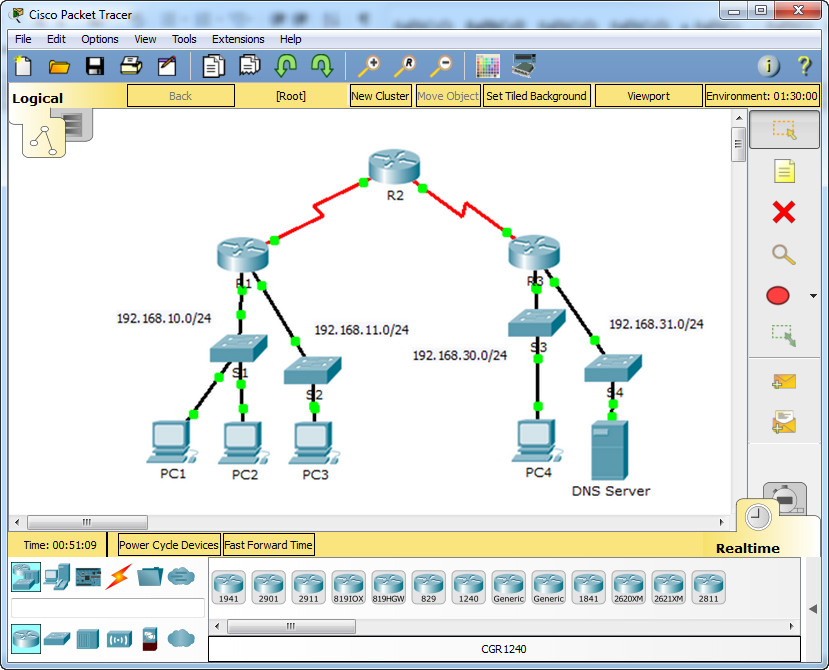
\includegraphics[width=0.75\textwidth]{packet_tracer}
    \caption{Nástroj Cisco Packet Tracer spustený v prostredí Windows}
    \cite{obr_packet_tracer}
    \label{obr:packet_tracer}
\end{figure}

\subsection{Dynamips/Dynagen}

Dynamips je open-source emulátor Cisco smerovačov na Linux/Windows \cite{dynamips}. Nástroj je v prevažnej mierie napísaný v jazyku C \cite{dynamips_github}. Podporuje iba výlučne vybrané Cisco smerovače \cite{dynamips}. Ovláda sa cez príkazový riadok. Portové čísla na vzdialený prístup sa zariadeniam prideľujú manuálne. Vzdialený prístup k zariadeniam v topológii je realizovaný protokolom \emph{telnet}. Na vytváranie topológii sa používa jednoduchý značkovací jazyk.

Nástroj Dynagen, ktorý slúži ako nadstavba nad platformou Dynamips, slúži na jednoduchšiu prácu s topológiami \cite{dynamips}. Topológie môže spravovať výlučne administrátor, pretože ani Dynamips, ani Dynagen nevedia rozlišovať rôzne typy používateľov. Počet topológii, ktoré môžu byť súčasne spustené je obmedzené iba výkonom servera. Na jednej topológii môžu pracovať aj viacerí študenti, tým že sa rozdelia portové čísla zariadení v topológii medzi študentov. Nástroj Dynamips umožňuje prepojiť topológiu so živou sieťou \cite{dynamips, dynamips_nil}. 

V súčasnosti sa o nástroj starajú vývojári nástroja GNS3 \cite{dynamips_github}. Na obrázku \ref{obr:dynamips_dynagen} je znázornený nástroj Dynagen.

\begin{figure}
    \centering
    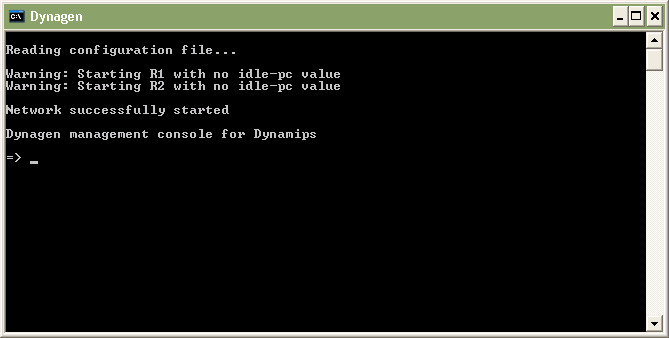
\includegraphics[width=0.75\textwidth]{dynamips_dynagen}
    \caption{Nástroj Dynagen spustený v prostredí Windows} \cite{obr_dynamips_dynagen}
    \label{obr:dynamips_dynagen}
\end{figure}

\subsection{WEB-IOU}

WEB-IOU, je simulačný nástroj pre platformu Linux, ktorý podporuje výlučne Cisco IOU platformu. Jeho hlavnou výhodou je podpora Cisco prepínačov, ktorá pri Dynamips/Dynagen chýba. Jeho autorom je Andrea Dainese \cite{webiou_github, webiou_unetlab_unetlabv2}.Nástroj je v prevažnej mierie napísaný v jazykoch PHP a JavaScript \cite{webiou_github}. Podporuje iba výlučne vybrané Cisco smerovače na platforme IOU - IOS on Unix \cite{webiou_firewall_cx}. Je vhodný na trénovanie pri certifikáciách CCNP a do istej miery aj CCIE. 

Spravuje sa cez príkazový riadok. Používateľovi je dostupné web rozhranie. Portové čísla na vzdialený prístup sa zariadeniam prideľujú automaticky. Vzdialený prístup k zariadeniam v topológii je realizovaný protokolom \emph{telnet}. Na vytváranie topológii sa používa jednoduchý značkovací jazyk \emph{NETMAP}. Topológie môže ktokoľvek, kto má prístup k web rozhraniu, pretože ani tento nástroj nevie rozlišovať rôzne typy používateľov. Počet topológii, ktoré môžu byť súčasne spustené je obmedzené iba výkonom servera. Napriek tomu môžu na jednej topológii môžu pracovať aj viacerí študenti rovnakým spôsobom, ako pri nástroji Dynamips/Dynalab. Nástroj WEB-IOU tiež umožňuje prepojiť topológiu so živou sieťou \cite{webiou_real_network}. 

V súčasnosti sa už nástroj nevyvíja. Na obrázku \ref{obr:webiou} je znázornené webové rozhranie nástroja WEB-IOU.

\begin{figure}
    \centering
    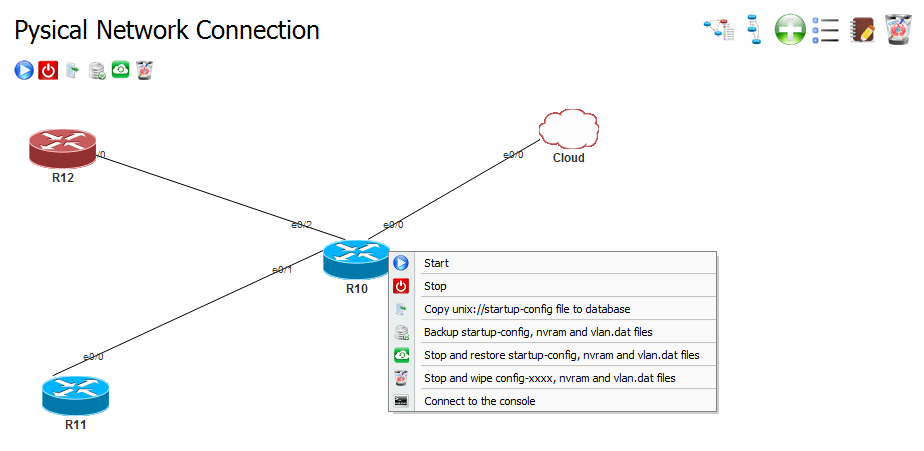
\includegraphics[width=0.75\textwidth]{webiou}
    \caption{Webové rozhranie nástroja WEB-IOU} \cite{obr_webiou}
    \label{obr:webiou}
\end{figure}

\subsection{Cisco VIRL}

VIRL, Virtual Internet Routing Lab, je komerčný simulačný nástroj sietí vyvíjaný spoločnosťou Cisco. Podporuje nielen Cisco smerovače a prepínače, ale aj zariadenia iných výrobcov, hoci ich integrácia nemusí byť jednoduchá. Výhodou oproti iným nástrojom je možnosť pridať podporované zariadenia do topológie ako LXC kontajner. Nevýhodou je, že nepodporuje Dynamips/Dynagen emuláciu, takže na ňom nie je možné využiť existujúce virtuálne zariadenia na katedre. Nástroj je postavený na platforme Linux (Debian) a je dostupný ako virtuálny stroj pre rôzne platformy. Je vhodný na trénovanie pri certifikáciách CCNP a do istej miery aj CCIE \cite{virl_cisco}. 

Spravuje sa cez príkazový riadok. Používateľovi je dostupné web rozhranie. Portové čísla na vzdialený prístup sa zariadeniam prideľujú automaticky \cite{virl_interfacett_1}. Vzdialený prístup k zariadeniam v topológii je realizovaný protokolmi \emph{telnet} a \emph{ssh}, po úprave aj \emph{vnc} \cite{virl_ciscoskills, virl_speaknetworks}. Na vytváranie topológii sa používa Nástroj \emph{VM Maestro}. Ten poskytuje možnosť, vopred si nakonfigurovať zariadenie podľa zvolených scenárov pomocou funkcie \emph{AutoNetkit}. Aj napriek tomu, že VIRL poskytuje pomerne podrobné možnosti na konfiguráciu zariadení a topológii, jeho používanie je pomerne obtiažne, hlavne pri vytváraní topológii \cite{virl_interfacett_1, virl_interfacett_2}. Cisco VIRL vie rozlišovať rôzne typy používateľov \cite{virl_cisco_features}. Počet topológii, ktoré môžu byť súčasne spustené je obmedzené iba výkonom servera. Napriek tomu môžu na jednej topológii môžu pracovať aj viacerí študenti rovnakým spôsobom, ako pri nástroji Dynamips/Dynalab \cite{virl_interfacett_2}. Nástroj tiež umožňuje prepojiť topológiu so živou sieťou \cite{virl_speaknetworks}. 

Nástroj v súčasnosti existuje iba vo verzii \emph{Personal Edition} s licenciou na 20 zariadení, čo výrazným spôsobom obmedzuje jeho využitie pri vyučovaní. V minulosti existovali aj verzie \emph{Personal Edition} s licenciou na 30 zariadení a \emph{Academic Edition}. Rozdiel medzi Personal a Academic Edition bol iba ten, že Academic Edition bol prístupný učiteľom a študentom za výhodnejšiu cenu. Podporované funkcionality boli zhodné v oboch verziách \cite{virl_edition_differences}. Na obrázkoch \ref{obr:virl_vmmaestro} a \ref{obr:virl_web} je v tomto poradí znázornený nástroj na vytváranie topológii VM Maestro a webové rozhranie Cisco VIRL.

\begin{figure}
    \centering
    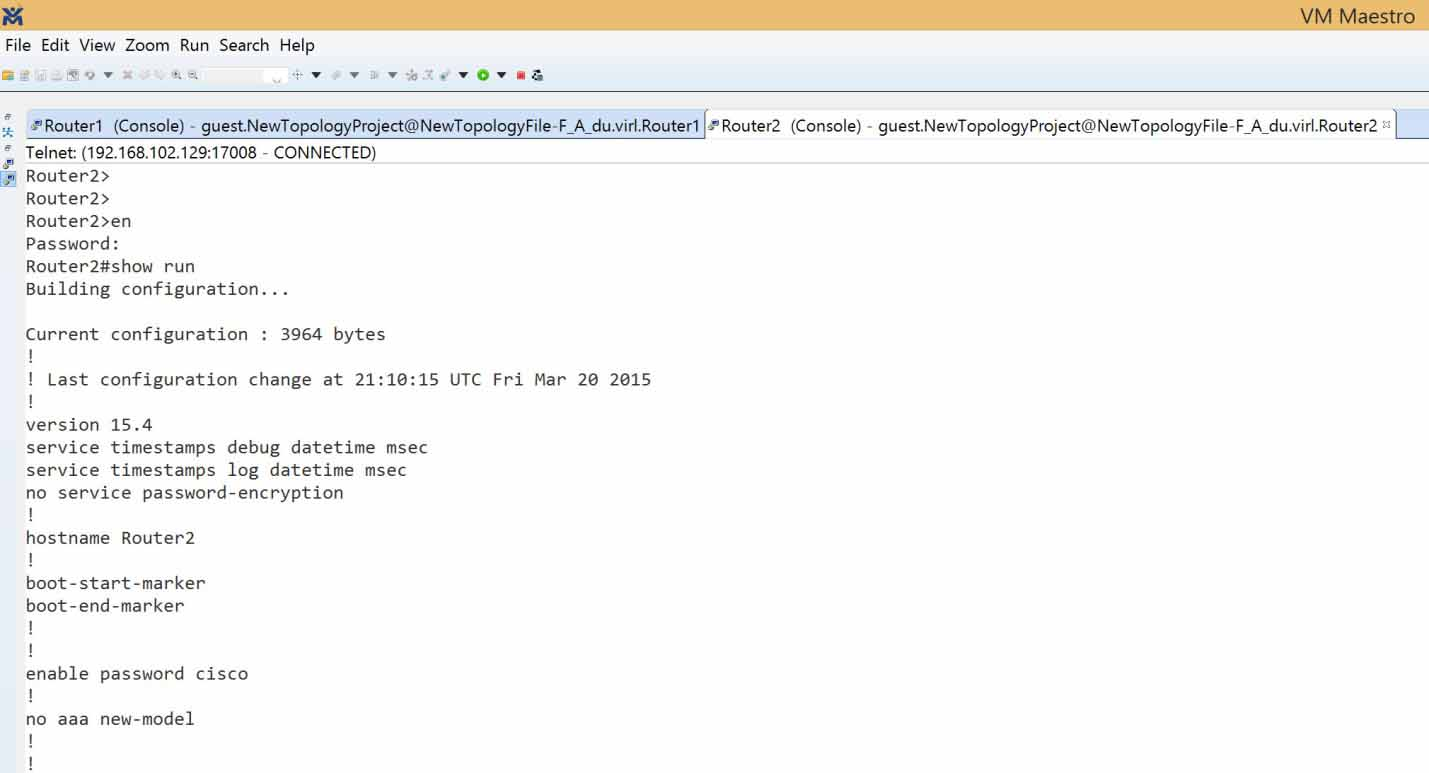
\includegraphics[width=0.75\textwidth]{virl_vmmaestro}
    \caption{VM Maestro} \cite{obr_virl_vmmaestro}
    \label{obr:virl_vmmaestro}
\end{figure}

\begin{figure}
    \centering
    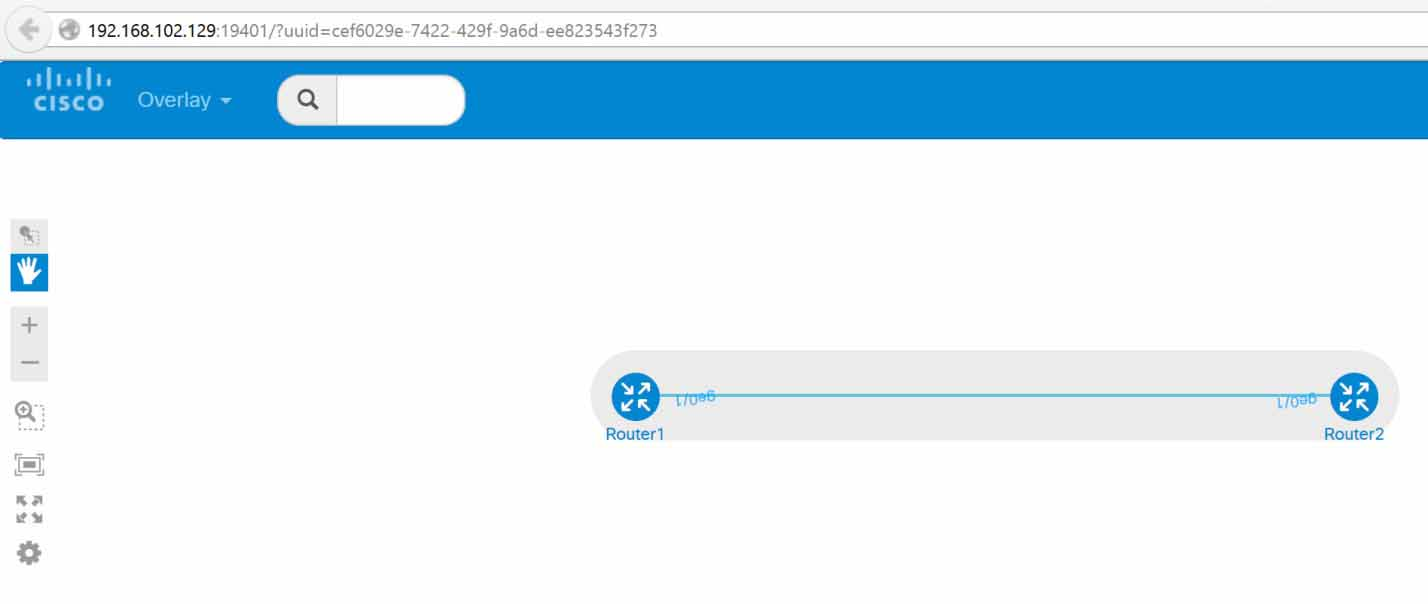
\includegraphics[width=0.75\textwidth]{virl_web}
    \caption{Cisco VIRL web rozhranie} \cite{obr_virl_web}
    \label{obr:virl_web}
\end{figure}

\subsection{ViRo v2}

ViRo, resp. ViRo v2, je virtuálne laboratórium vytvorený na Katedre informačných sietí. Nástroj vznikol ako výsledok diplomovej práce Ing. Petra Hadača, pričom pokračoval v predchádzajúcej verzii nástroja, ViRo v1. Nástroj je postavený na platforme Linux. Využíva technológie tzv. \emph{LAMP Stack} servera: Linux, Apache, MySQL, PHP (Drupal). Využíva virtualizáciu pomocou QEMU/KVM a Dynamips. Jeho hlavnou výhodou je možnosť rezervovať si topológiu. Potenciálnou nevýhodou je, že nepodporuje platformu Cisco IOL. Ďalšou možnou nevýhodou je, že stavia na platforme Drupal, ktorého popularita je pomerne nízka \cite{stackoverflow_survey}.

Spravuje sa prostredníctvom web rozhrania, SSH alebo VNC prístupu. Používateľom s rolou \emph{učiteľ} a \emph{študent} je dostupné webové rozhranie. Portové čísla na vzdialený prístup sa zariadeniam dajú nastaviť manuálne. Vzdialený prístup k zariadeniam v topológii je realizovaný viacerými spôsobmi: pomocou nástroja \emph{virsh}, aplikáciou \emph{Virtual Machine Manager} prístupnou cez \emph{vnc}, \emph{noVNC} serverom alebo SSH tunelom. Vytváranie topológii a správu zariadení sa používa grafický nástroj \emph{Virtual Machine Manager}. Topológie môže vytvárať iba používateľ s rolou  \emph{učiteľ} alebo \emph{administrátor}, keďže nástroj ViRo vie rozlišovať rôzne typy používateľov. Počet topológii, ktoré môžu byť súčasne spustené je obmedzené iba výkonom servera. Napriek tomu môžu na jednej topológii môžu pracovať aj viacerí študenti rovnakým spôsobom, ako pri nástroji Dynamips/Dynalab. Nástroj umožňuje prepojiť topológiu so živou sieťou pomocou \emph{bridge} rozhrania \cite{viro_hadac}.

\subsection{UNetLab}

UNetLab, Unified Networking Lab, skrátene UNL, je open-source  simulačný nástroj pre platformu Linux, ktorý integruje všetky vyššie uvedené technológie najednom mieste: Dynamips, Cisco IOU aj zariadenia tretích strán (QEMU). Nástroj je postavený na platforme Linux. Jeho autorom je Andrea Dainese. V prevažnej mierie je napísaný v jazykoch PHP a JavaScript \cite{webiou_unetlab_unetlabv2, unetlab_github}. Je vhodný nielen na trénovanie pri Cisco certifikáciách, ale aj na testovanie kompatibility rôznych výrobcov.

Spravuje sa cez príkazový riadok. Používateľovi je dostupné web rozhranie. Portové čísla na vzdialený prístup sa zariadeniam prideľujú automaticky. Vzdialený prístup k zariadeniam v topológii je realizovaný protokolom \emph{telnet} alebo \emph{vnc}. Topológie sa vytvárajú vo webovom rozhraní prepájaním uzlov medzi sebou pomocou myši, pričom sa na pozadí sa generuje súbor v značkovacom jazyku \emph{NETMAP}. Topológie môže ktokoľvek, kto má prístup k web rozhraniu, pretože ani tento nástroj nevie rozlišovať rôzne typy používateľov, hoci v istej verzii nástroja táto funkcia bola podporovaná \cite{unetlab_github}. Počet topológii, ktoré môžu byť súčasne spustené je obmedzené iba výkonom servera. Napriek tomu môžu na jednej topológii môžu pracovať aj viacerí študenti rovnakým spôsobom, ako pri nástroji Dynamips/Dynalab. Jeden používateľ môže mať otvorenú práve jednu topológiu. Topológia sa dá zatvoriť až vtedy, keď v nej nie sú spustené žiadne zariadenia. Nástroj UNetLab tiež umožňuje prepojiť topológiu so živou sieťou pomocou \emph{bridge} rozhrania \cite{webiou_real_network}.

Vývoj tohto nástroja bol zastavený. UNetLab ďalej vyvíjala iná skupina vývojárov, ktorý nástroj premenovala na EVE-ng a migrovala ho z platformy Ubuntu 14.04 na Ubuntu 16.04. Jeho pôvodný autor následne začal s vývojom ďalšej verzie nástroja UNetLab, UNetLabv2. Na obrázku \ref{obr:unetlab_web} je znázornené webové rozhranie nástroja UNetLab.

\begin{figure}
    \centering
    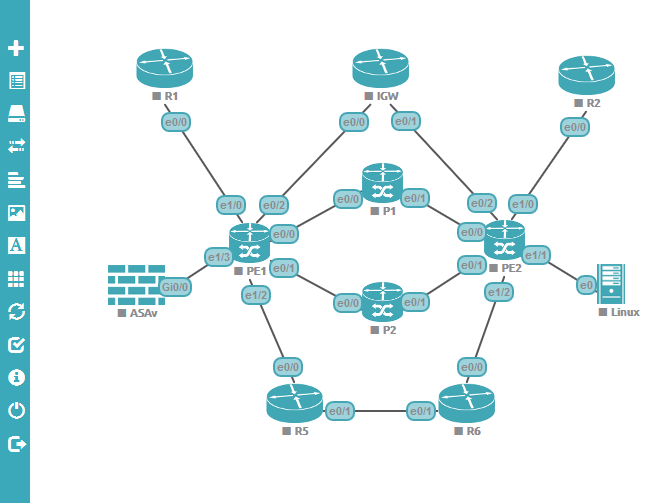
\includegraphics[width=0.75\textwidth]{unetlab_web}
    \caption{Webové rozhranie nástroja UNetLab}
    \cite{obr_unetlab_web}
    \label{obr:unetlab_web}
\end{figure}

\subsection{EVE-ng}
\label{chap:virt_lab_eve_ng}

EVE-ng je simulačný nástroj sietí, ktorý vznikol ako klon a nasledovník nástroja UNetLab. Celkovou funkcionalitou, až na niektoré zmeny, napr. použitie MySQL namiesto SQLite, pridaná podpora pre ďalšie zariadenia), a vzhľadom webového rozhrania sa preto veľmi podobá na svojho predchodcu. Nástroj je postavený na platforme Linux a vyvíjaný prevažne v jazykoch JavaScript a PHP. Web rozhranie je realizované ako webová aplikácia s použitím framework nástroja \emph{Angular JS} a \emph{Twitter Bootstrap} \cite{eve_ng_technologies}.

EVE-ng sa v priebehu marca 2018 rozdelilo na tri verzie: Community, Professional a Learning Centre. Community verzia je open-source, aj keď \emph{gitlab} repozitár bol neprístupný pre verejnosť v priebehu novembra/decembra 2017. Napriek tomu sú na serveri všetky súbory prístupné a upravovateľné. Túto verziu je možné slobodne šíriť a upravovať. Verzia Professional obsahuje niektoré funkcionality, ktoré uľahčujú prácu s nástrojom, ale vývojári sa rozhodli spoplatniť ju. Learning Centre verzia obsahuje funkcionality na nasadenie do produkčného prostredia, ako je napr. rozdelenie používateľov do používateľských rolí. Podrobný zoznam podporovaných funkcii v jednotlivých verziách je dostupný v \cite{eve_ng_versions_table} a \cite{eve_ng_versions_list}.

Vzhľad webového rozhrania EVE-ng je znázornený na obrázku \ref{obr:eve_ng_web}. Rozdiely jednotlivých verzii EVE-ng sú znázornené v tabuľke \ref{tab:eve_ng_versions}.

\begin{figure}
    \centering
    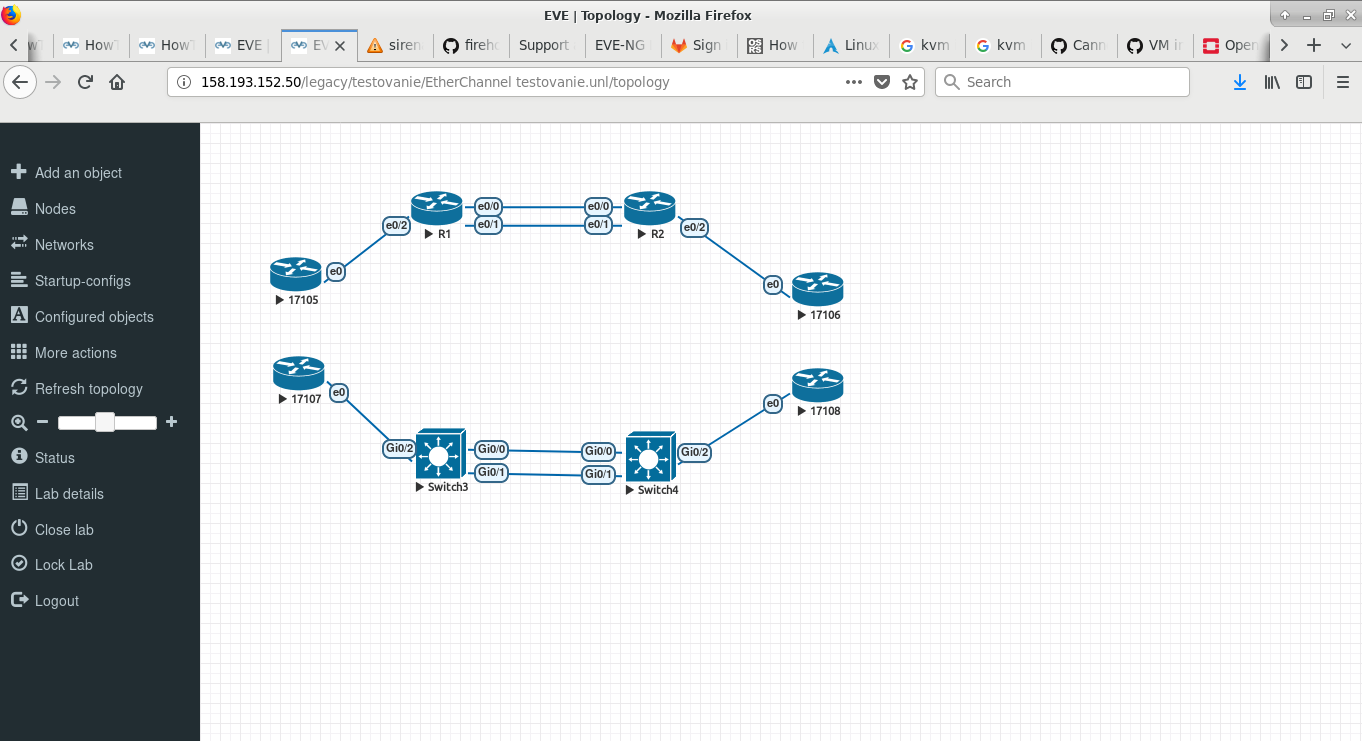
\includegraphics[width=0.75\textwidth]{eve_ng_web}
    \caption{Webové rozhranie nástroja EVE-ng}
    \label{obr:eve_ng_web}
\end{figure}

\begin{longtable}{| m{3cm} | m{2cm} | m{2cm} | m{2cm} | m{4cm} |}
\caption{Porovnanie EVE-ng verzii}
\cite{eve_ng_versions_table}
\label{tab:eve_ng_versions} \\
\hline
Features/Edition                                      & Community         & Professional    & Learning Center      & Description                                                                                                   \\ \hline
Price                                                 & Free              & 99 EUR w/o VAT  & 99 EUR + Added Roles &                                                                                                               \\ \hline
User's roles                                          & admin only        & admin only      & admin, user, editor  & Restrictions of the EVE usage, WEB UI, per user based                                                         \\ \hline
Lock user per folder                                  & No                & No              & Yes                  & User cannot see other EVE folders, only his own                                                               \\ \hline
Lock user edit rights                                 & No                & No              & Yes                  & User cannot edit labs, images etc                                                                             \\ \hline
Shared Lab Folder                                     & No                & No              & Yes                  & Shared lab folder visible for all users                                                                       \\ \hline
User's account validity ( 1/4 Hour accuracy )         & No                & No              & Yes                  & Ability to set calendar validity for account, Date and time ( From -\textgreater To )                         \\ \hline
Lab Timer                                             & No                & Yes             & Yes                  & Timer for Lab training                                                                                        \\ \hline
Running labs folder                                   & No                & Yes             & Yes                  & User can run more than one lab. Running labs will appear in special running labs folder. Per user based       \\ \hline
Node limit per lab                                    & 63                & 1024            & 1024                 & Limit of nodes to run per lab                                                                                 \\ \hline
TCP ports                                             & fixed 128 per POD & Dynamic 1-65000 & Dynamic 1-65000      & Automatic TCP port choose for telnet session                                                                  \\ \hline
Local Wireshark capture                               & Yes               & No              & No                   & Local wrapper using ssh and root password to the EVE                                                          \\ \hline
Local Telnet client                                   & Yes               & Yes             & Yes                  & Local wrapper using locally installed telnet client                                                           \\ \hline
Local VNC client                                      & Yes               & Yes             & Yes                  & Local wrapper using locally installed vnc client                                                              \\ \hline
Wireshark integrated                                  & No                & Yes             & Yes                  & Docker integrated wireshark                                                                                   \\ \hline
Docker container support                              & No                & Yes             & Yes                  & Docker container support                                                                                      \\ \hline
Running nodes interface connections (hot connections) & No                & Yes             & Yes                  & Hot/live nodes interface connection                                                                           \\ \hline
NAT Cloud                                             & No                & Yes             & Yes                  & Integrated NAT cloud, connect node to the internet. NAT to the EVE management interface DHCP 169.254.254.0/24 \\ \hline
HTML console without Wireshark capture                & Yes               & No              & No                   & HTML console                                                                                                  \\ \hline
HTML console with Wireshark capture                   & No                & Yes             & Yes                  & HTML wireshark capture                                                                                        \\ \hline
HTML Desktop Console                                  & No                & Yes             & Yes                  & Integrated Docker PC management                                                                               \\ \hline
Multi startup configuration choose per lab            & No                & Yes             & Yes                  & Option to create and boot lab from different startup configurations, multi startup config                     \\ \hline
Export/Import configs or config packs to local PC     & No                & Yes             & Yes                  & Option import and export single config or config packs to the lab                                             \\ \hline  
\end{longtable}

Z tabuľky vyplýva, že verzie \emph{Community} je ako jediná bezplatná. Najväčšími výhodami ostatných verzii je rozdelenie používateľov do používateľských rolí (iba v \emph{Learning Centre}), zatvorenie topológie s už spustenými zariadeniami, prehľad zatvorených topológii so spustenými zariadeniami a zvýšený limit na počet spustených zariadení pre topológiu.

Doplnením a rozšírením funkcionality EVE-ng Community verzie je venovaná kapitola \ref{chap:eve_ng_uprava_zdroj_kodov} - \nameref{chap:eve_ng_uprava_zdroj_kodov}

\subsection{GNS3}

GNS3, Graphical Network Simulator 3, je open-source sieťový simulátor sietí. Integruje všetky virtualizačné technológie najednom mieste: Dynamips, Cisco IOU aj zariadenia tretích strán (QEMU). Od verzie 1.5 sú v GNS3 podporované aj Docker kontajnery, čo je veľkou výhodou oproti iným nástrojom, pretože Docker kontajnery potrebujú menej systémových prostriedkov \cite{gns3_docker}.

GNS3 sa skladá z klientskej a serverovej časti. Klientská časť pozostáva z aplikácie \emph{GNS3 Client} a je celá napísaná v jazyku Python \cite{gns3_gui_github}. Klientská aplikácia je multiplatformová t.j. je kompatibilná s platformami Windows, Linux a macOS. Existuje aj klientská webová aplikácia \emph{gns3-web} \cite{gns3_web_github}.

Serverová časť môže byť realizovaná ako serverová aplikácia \emph{GNS3 Server}, ako virtuálny stroj \emph{GNS3 VM} alebo ako vzdialený server.

Serverová aplikácia \emph{GNS3 Server} sa spustí predvolene pri spustení klientskej aplikácie. Rovnako, ako GNS3 klientská aplikácia, aj serverová aplikácia je napísaná celá v jazyku Python \cite{gns3_server_github}.

GNS3 VM aj vzdialený server je postavený na platforme Linux. Vzdialený server nemusí nutne byť fyzický server, na ktorom je nasadený GNS3 server. Môže byť v ľubovoľnom virtualizačnom nástroji, napr. vo VMware. VMware je odporúčaná voľba pre tento virtualizačný nástroj, pretože podporuje vnorenú virtualizáciu, čo VirtualBox doposiaľ nepodporuje \cite{nested_virtualization}.

GNS3 VM resp. vzdialený server sa spravuje cez príkazový riadok. Používateľovi je dostupná klientská aplikácia. Portové čísla na vzdialený prístup sa zariadeniam prideľujú automaticky, avšak je možné manuálne meniť rozsah, v akom sa majú portové čísla automaticky prideľovať, dokonca umožňuje aj manuálnu zmenu čísla portu pre jednotlivé zariadenia \cite{gns3_console_ports, gns3_console_ports_remote}. Vzdialený prístup k zariadeniam v topológii je realizovaný protokolom \emph{telnet}, \emph{vnc} alebo\emph{rdp}. Topológie sa vytvárajú v klientskej aplikácii prepájaním uzlov medzi sebou pomocou myši. V predvolenom nastavení sú všetky topológie zdieľané a môže ich meniť ktokoľvek, kto má prístup k web rozhraniu, pretože v predvolenom nastavení nástroj nevie rozlišovať rôzne typy používateľov ani ich izolovať. Počet topológii, ktoré môžu byť súčasne spustené je obmedzené iba výkonom servera. Napriek tomu môžu na jednej topológii môžu pracovať aj viacerí študenti tým, že si otvoria rovnaký projekt na vzdialenom serveri. Zmeny v takejto zdieľanej topológii sa prejavia okamžite všetkým používateľom. Jeden používateľ môže mať spustených aj viacero topológii, v klientská aplikácia však dovoľuje pracovať iba s jednou naraz. Topológia sa dá kedykoľvek zatvoriť. Aj GNS3, podobne ako aj ďalšie nástroje, umožňuje prepojiť topológiu so živou sieťou pomocou \emph{bridge} rozhrania.

Vývoj tohto nástroja stále pokračuje. Na obrázku \ref{obr:gns3_client} je znázornená klientská aplikácia GNS3 Client.

\begin{figure}
    \centering
    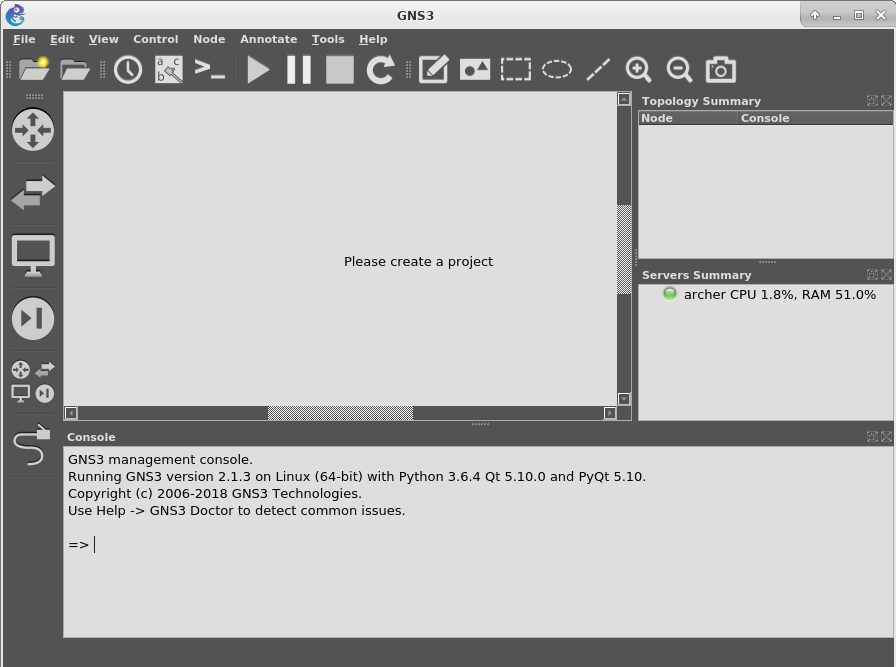
\includegraphics[width=0.75\textwidth]{gns3_client}
    \caption{Klientská aplikácia GNS3}
    \label{obr:gns3_client}
\end{figure}

\subsection{UNetLabv2}

UNetLabv2 je nasledovníkom nástroja UNetLab. Je postavený na platforme Docker kontajnerov. Jednotlivé úlohy sú distribuované naprieč kontajnermi. To zaisťuje lepšiu škálovateľnosť pri zachovaní rovnakej funkcionality. Zatiaľ ešte nie je verejne nedostupný.

Architektúra nástroja UNetLabv2 je znázornená na obrázku \ref{obr:unetlabv2_arch}

\begin{figure}
    \centering
    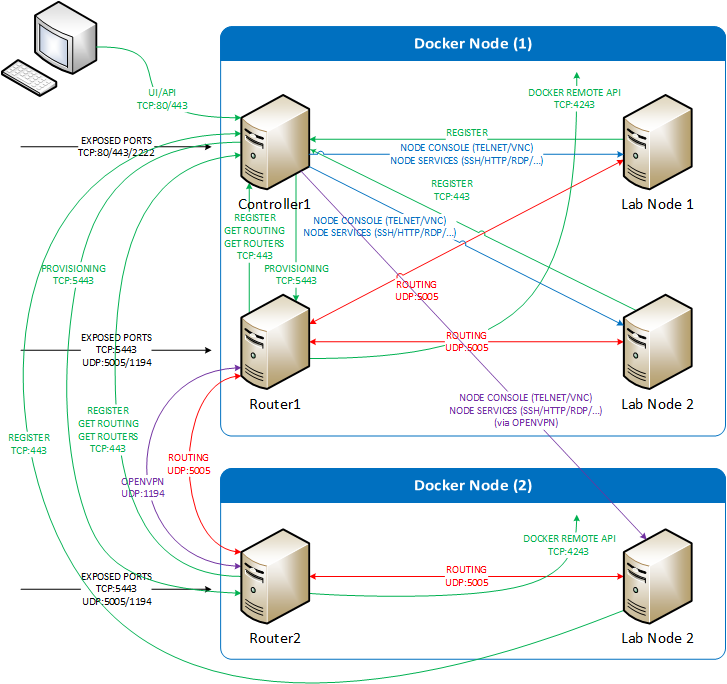
\includegraphics[width=0.75\textwidth]{unetlabv2_arch}
    \caption{Architektúra nástroja UNetLabv2} \cite{obr_unetlabv2_arch}
    \label{obr:unetlabv2_arch}
\end{figure}

\section{Vyhodnotenie}

Z vyššie uvedených nástrojov má zmysel zaoberať sa nástrojmi EVE-ng a GNS3 z nasledovných dôvodov:
\begin{itemize}
    \item Open-source vývoj oboch nástrojov umožňuje ich používanie bez poplatkov, obáv o porušenie licenčných podmienok a poskytuje možnosť upravovať ich podľa vlastných požiadaviek.
    \item Podpora zariadení od rôznych výrobcov.
    \item Jednoduché ovládanie.
\end{itemize}

V priebehu projektu sme sa preto zamerali na nástroje GNS3 a EVE-ng. Počas neho sa však ukázalo, že GNS3 nie je vhodná pre vzdialené použitie, preto sme sa týmto nástrojom ďalej nezaoberali. V čase skúmania bol nástroj GNS3 vo verzii 1.5.3. Keď sme skúšali použiť GNS3 ako vzdialený server, klientská aplikácia sa na GNS3 vzdialený server nevedela pripojiť, hoci sme postupovali podľa návodov na GNS3 stránke a pri testovaní nestála v pripojení na server žiadna prekážka napr. firewall.

{\huge TODO - pridať širšie porovnanie EVE-ng a GNS3 - viď súbor gns3 vs eve-ng.txt}

\begin{longtabu} to \textwidth {| X[5.0,cm] | X[5.0,cm] | X[5.0,cm] |}
\caption{Porovnanie GNS3 a EVE-ng}
\label{tab:gns3_eve_ng_porovnanie} \\
\hline
    & \textbf{GNS3} & \textbf{EVE-ng} \\
\hline
    \textbf{Výhody}
    &
        \begin{itemize}
            \item bla
            \item ble
        \end{itemize}    
    &
        \begin{itemize}
            \item hurr
            \item durr
        \end{itemize}  \\
\hline
    \textbf{Nevýhody} & & \\
\hline
\end{longtabu}

GNS3 od vydania stabilnej verzie 2.0.0 opravila problém s nasadením ako vzdialený server. Avšak vtedy som už začal s hlbším skúmaním EVE-ng. Skúmanie dvoch nástrojov naraz do hĺbky by bolo časovo veľmi náročné. GNS3 slúžila počas skúmania ako podporný nástroj pre pochopenie rôznych technických súčastí virtualizácie sieťových zariadení.

Vo zvyšku diplomovej práce sa zaoberám nástrojom EVE-ng a jeho nasadením do vyučovania na katedre.

\chapter{EVE-ng}
\label{chap:eve_ng}

EVE-ng je virtuálne sieťové laboratórium skladajúcej sa zo serverovej časti postavenej na platforme Linux, konkrétne ako tzv. LAMP server, a klientskej časti, ktorú tvorí webová aplikácia, ako je už spomenuté v kapitole \ref{chap:nastroje_pre_siet_virt} v časti \ref{chap:virt_lab_eve_ng}. V tejto kapitole bude opísaný proces nasadzovania EVE-ng servera do sieťovej infraštruktúry katedry: jeho inštalácie, následnej úpravy a základnej administrácie EVE-ng servera. Všetky kroky sú podrobne opísané v návodoch na priloženom CD v adresári \emph{eve-ng}.

Po inštalácii servera je potrebné do určitej miery upraviť aj konfiguráciu klientských počítačov, ktoré budú EVE-ng server používať. Úpravám na klientskej strane sa venujem v bode \ref{item:vzdialeny_pristup} v časti \ref{chap:vytvorenie_topo_eve-ng} - \nameref{chap:vytvorenie_topo_eve-ng}.




\section{Inštalácia}

EVE-ng bol inštalovaný a testovaný na dvoch platformách:

\begin{itemize}[noitemsep]
    \item VMware Workstation Player
    \item Fyzický server
\end{itemize}

Parametre VMware virtuálneho stroja a fyzického servera sú uvedené v tabuľke \ref{tab:server_parameters}. V oboch prípadoch bol EVE-ng server nasadený do DMZ zóny, preto v riadku \emph{IP adresa} uvádzam len posledný oktet ich IPv4 adries, keďže IP adresa DMZ siete je na katedre známa.

\begin{longtabu} to \textwidth {| X[5.0,cm] | X[5.0,cm] | X[5.0,cm] |}
\caption{Parametre EVE-ng serverov}
\label{tab:server_parameters} \\
\hline
    \textbf{Parametre \textbackslash~ Server} & \textbf{VMware} & \textbf{Fyzický server} \\
\hline
    \textbf{CPU} & 16 & 8 \\
\hline
    \textbf{Operačná pamäť (GB)} & 16 & 48 \\
\hline
    \textbf{EVE-ng verzia} & 2.0.3-80 & 2.0.3-86 \\
\hline
    \textbf{IP adresa} & .49 & .50 \\
\hline
\end{longtabu}

\noindent
Uvedené tvrdenia platia pre EVE-ng vo vydaní \emph{Community Edition} vo verzii 2.0.3-86.

\noindent
Postup inštalácie EVE-ng servera môžeme zhrnúť do týchto krokov:

\begin{enumerate}[noitemsep]
    \item Vytvorenie vzdialenej pracovnej plochy
    \item Inštalácia Ubuntu Server 16.03
    \item Konfigurácia Ubuntu Server
    \item Inštalácia EVE-ng do Ubuntu Server
    \item Konfigurácia EVE-ng servera
\end{enumerate}

\noindent   
Konfigurácia EVE-ng servera zahŕňala:

\begin{enumerate}[noitemsep]
    \item Obnovenie súborov a adresárov
    \begin{itemize}[noitemsep]
        \item Skripty
        \item Zariadenia
        \item Databázy
    \end{itemize}
    \item Automatizácia zálohovania
    \item Pridanie Cisco IOL/IOU licencie
    \item Zabezpečenie servera
    \begin{itemize}[noitemsep]
        \item Systém
        \item SSH
        \item Webový server
    \end{itemize}
    \item Úprava šablón
    \item Úprava zdrojových kódov
\end{enumerate}

Inštalačný proces pre obe platformy, virtuálnu aj fyzickú, bol takmer zhodný, líšil sa iba v úvodných krokoch. Pri inštalácii pre VMware bolo totiž potrebné na server, na ktorom bol VMware nainštalovaný pridať VNC prístup a doplniť grafické prostredie, aby bolo možné ovládať grafické rozhranie VMware Player a spustiť virtuálny stroj. Pre VMware Player to bolo jediným riešením, ako vytvoriť virtuálny EVE-ng server.

Rozdielov medzi oboma inštaláciami je niekoľko. Prvým z nich je už spomenutá verzia. VMware inštalácia má nižšiu verziu, pretože bola nainštalovaná skôr. VMware inštalácia slúžila na prvotné odladenie a pilotné nasadenie do vyučovania. Nebola v nej vykonaná takmer žiadna dodatočná konfigurácia, okrem importu zariadení pre topológie.

Následná inštalácia EVE-ng na fyzický server vychádzala zo skúseností získaných z inštalácie EVE-ng do VMware prostredia. EVE-ng fyzický server bol odladený a do veľkej miery testovaný. Testovaniu zariadení v EVE-ng sa venujem v kapitole \ref{chap:testovanie_zariadeni} - \nameref{chap:testovanie_zariadeni}.

Nasadzovaniu jednotlivých EVE-ng serverov sa venujem v kapitole \ref{chap:nasadenie_do_vyucovania} - \nameref{chap:nasadenie_do_vyucovania}. Obnovovanie súborov a adresárov môžeme preskočiť, ak predtým ešte nebola vytvorená záloha príslušným zálohovacím skriptom. Zálohovaniu sa venujem v časti \ref{chap:zalohovanie} - \nameref{chap:zalohovanie}.

Pridanie Cisco IOL/IOU licencie je dôležitým krokom, bez ktorého by sme neboli schopní spúšťať Cisco IOL/IOU zariadenia. Význam týchto zariadení bude vysvetlený v kapitole \ref{chap:testovanie_technologii} - \nameref{chap:testovanie_technologii}.

Zabezpečenie servera spočívalo hlavne v zabezpečení operačného systému, SSH prístupu a webového servera.

Zabezpečenie operačného systému obsahovalo vytvorenie štandardného používateľského konta so \emph{sudo} oprávneniami. Ten sa bude používať namiesto \emph{root} používateľa, čím bude zaistená vyššia bezpečnosť pri používaní systému.

Zabezpečenie SSH prístupu zahŕňalo v zablokovanie \emph{root} používateľa, explicitné definovanie povolených používateľov a skupín, vygenerovanie SSH kľúčov a vypnutie autentifikácie heslom. Autentifikácia SSH kľúčmi má aj tú výhodu, že oproti autentifikácii heslom nie je nutné zadávať heslo, čím odpadá aj nutnosť pamätať si ho. Každý počítač, ktorý by chcel EVE-ng server používať, by si musel svoj verejný SSH kľúč nahrať na server k danému používateľskému účtu. Rozhodli sme sa ale, že pre obidva servery bude ponechaná autentifikácia heslom.

Zabezpečenie webového servera Apache sa skladalo z vygenerovania SSL certifikátu a aktivácie protokolu HTTPS a presmerovania požiadaviek z HTTP na protokol HTTPS. Webový server však nie je zabezpečený na ani jednom serveri, pretože bolo potrebné odchytávať komunikáciu a nezašifrované vymieňané správy medzi klientom a EVE-ng serverom, pre potreby rozširovania funkcii v EVE-ng, ktorým sa venujem v časti \ref{chap:eve_ng_uprava_zdroj_kodov} - \nameref{chap:eve_ng_uprava_zdroj_kodov}.

Na serveri bola bola vykonaná aj úprava šablón, aby používateľ pri vytváraní topológie nemusel premýšľať nad technickými parametrami zariadenia, ktoré do topológie pridáva, ale na vyučovanú problematiku. Tak sa vytváranie topológii aj samotné vyučovanie stane plynulejším. Každé zariadenie, ktoré je možné do topológie pridať, si totiž načíta svoje technické parametre zo súboru zvaného šablóna. V šablóne môže byť pre zariadenie definovaný napr. počet pridelených jadier CPU, maximálne množstvo alokovateľnej operačnej pamäte, spúšťacie parametre zariadenia a pod. Úpravy šablón boli vykonané na základe testovania vybraných zariadení, ktoré opisujem v kapitole \ref{chap:testovanie_zariadeni_benchmark} - \nameref{chap:testovanie_zariadeni_benchmark}.




\section{Úprava nástroja EVE-ng}
\label{chap:eve_ng_uprava_zdroj_kodov}

EVE-ng muselo byť upravené aj v zdrojových kódoch, aby sa nástroj dal použiť aj vo vyučovaní. Nižšie sú uvedené úspešne vykonané zmeny.




\subsection{Metodika}

Na to, aby sme mohli odhadnúť, ktoré časti nástroja EVE-ng treba upraviť, sme použili nástroje \emph{Wireshark} a \emph{grep}.

Nástroj Wireshark slúžil na odchytávanie vymieňaných správ prostredníctvom REST API. Keďže webový server nebol zašifrovaný a používal HTTP protokol, mohli sme skúmať tieto správy v nezašifrovanom texte. Následne sme hľadali číselný kód správy v súboroch vo webovom adresári EVE-ng. To nám umožnilo spresniť odhad na tie časti zdrojového kódu, ktorých zmena by s veľkou pravdepodobnosťou mohla vyriešiť daný problém.




\subsection{Sprístupnenie používateľských rolí}
\label{chap:eve_ng_pouzivatelske_role}

V EVE-ng Community Edition je pre používateľov dostupná iba jedna používateľská rola \mbox{\emph{admin}}, čiže administrátor. Je to tak preto, lebo \emph{Community} verzia je určená pre osobné použitie, kde sa nepredpokladá viac používateľov, než je používateľ sám. Takéto správanie však nie je vhodné pre nasadenie do vyučovacieho procesu.

Odchytili sme preto správy pri úprave ľubovoľného používateľa. Zistili sme, že sa o.i. posiela aj správa \\
\texttt{Successfully listed user roles (60041)}. Po vyhľadaní výskytu kódu tejto správy v súboroch webového adresára sa ukázalo, že sa vyskytuje aj v súbore \\
\texttt{/opt/unetlab/html/includes/functions.php}.

Na sprístupnenie ďalších používateľských rolí, \emph{editor} - učiteľ a \emph{user} - používateľ resp. študent, bolo potrebné ich odkomentovať z funkcie \texttt{listRoles} v spomenutom súbore.

To vo web rozhraní sprístupnilo v dialógovom okne na vytvorenie a úpravu používateľa ďalšie používateľské role (obrázok \ref{obr:eve_ng_pouzivatelia_dialog}).

\begin{figure}
    \centering
    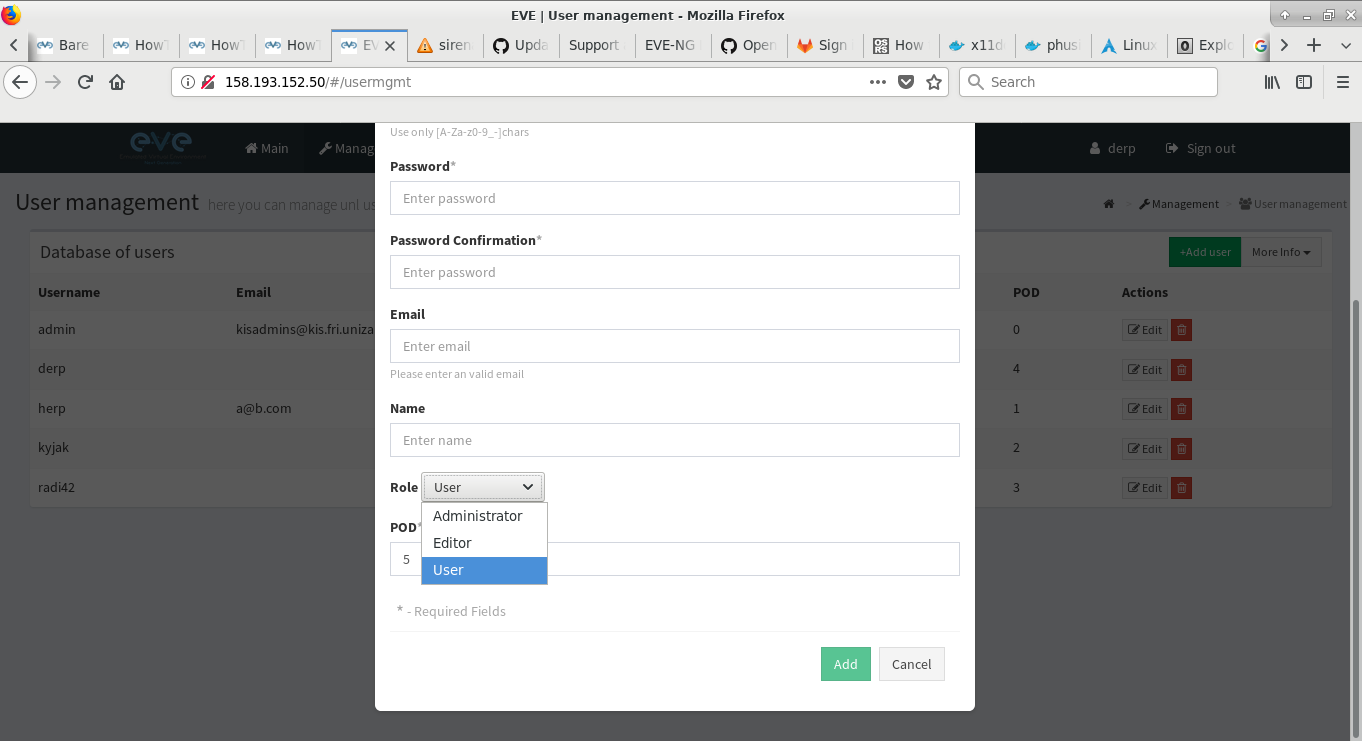
\includegraphics[width=0.75\textwidth]{eve_ng_pouzivatelia_dialog}
    \caption{Dialógové okno na vytvorenie a úpravu používateľa}
    \label{obr:eve_ng_pouzivatelia_dialog}
\end{figure}

Po vytvorení používateľa s inou rolou než \emph{admin}, napr. \emph{user}, sa vo web rozhraní v zozname používateľov stále zobrazujú ako \emph{admin}, hoci v MySQL databázi sú uložení pod správnou rolou v stĺpci \texttt{role} (obrázok \ref{obr:eve_ng_pouzivatelia_mysql}).

\begin{figure}
    \centering
    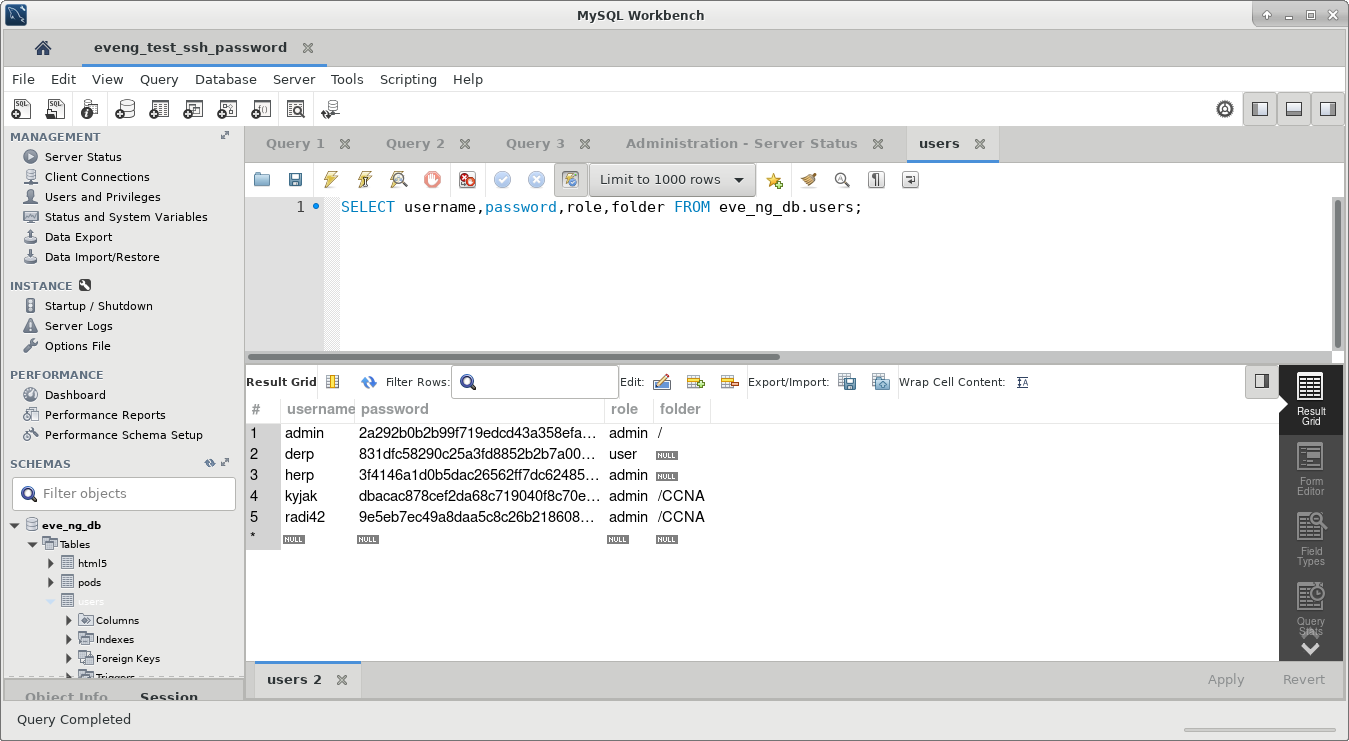
\includegraphics[width=0.75\textwidth]{eve_ng_pouzivatelia_mysql}
    \caption{Zoznam používateľov v MySQL databázi}
    \label{obr:eve_ng_pouzivatelia_mysql}
\end{figure}

Zachytená komunikácia obsahovala aj záznam so správou \\
\texttt{Successfully listed users (60040)} (obrázok \ref{obr:eve_ng_60040}),
ktorej kód sa nachádzal aj v súbore \\
\texttt{/opt/unetlab/html/includes/api\_uusers.php}.

\begin{figure}
    \centering
    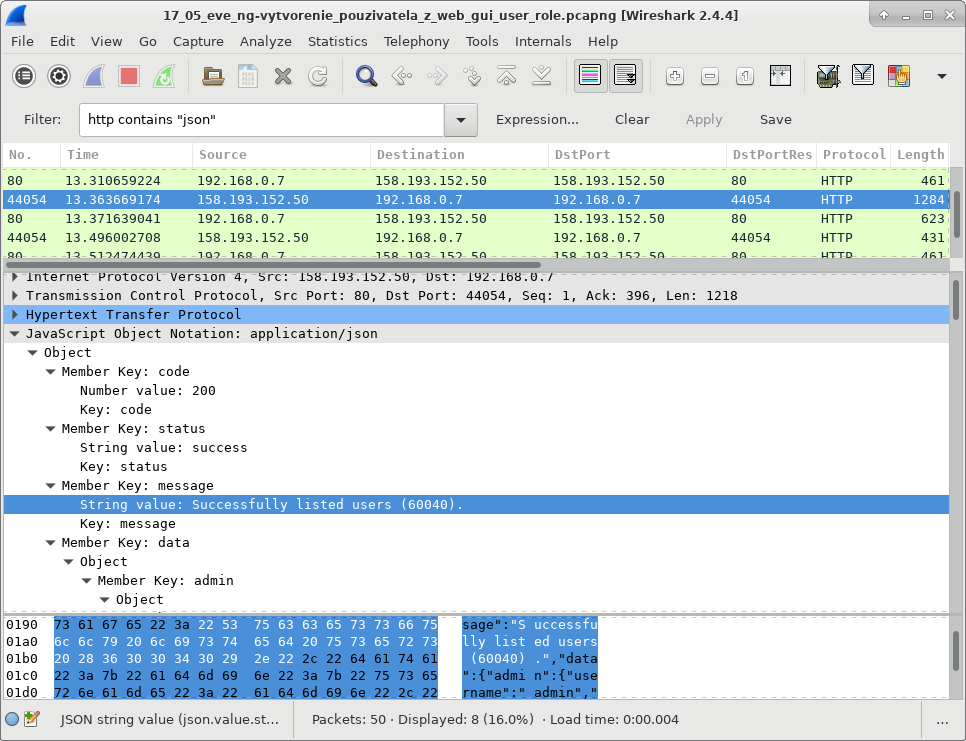
\includegraphics[width=0.75\textwidth]{eve_ng_60040}
    \caption{Správa 60040 - úspešné odoslanie zoznamu používateľov zo servera}
    \label{obr:eve_ng_60040}
\end{figure}

Riešenie spočívalo v úprave funkcii \texttt{apiGetUUser} a \texttt{apiGetUUsers} v spomenutom súbore. Prvá spomenutá funkcia sa stará o získanie informácii o jednom používateľovi, ďalšia o získanie atribútov všetkých používateľov z MySQL databázy. V oboch funkciách sa však vyskytovala rovnaká chyba, a síce, že používateľská rola sa v príkaze \emph{SELECT} napevno prepisovala na rolu \emph{admin}.

Stačilo v týchto príkazoch prepísať názov používateľskej role z pevnej hodnoty \emph{admin} na názov stĺpca používateľskej role t.j. \texttt{role}.

Po vykonanej úprave sa aj vo webovom zozname používateľov zobrazovala ich správna rola (obrázok \ref{obr:eve_ng_pouzivatelia_web}).

\begin{figure}
    \centering
    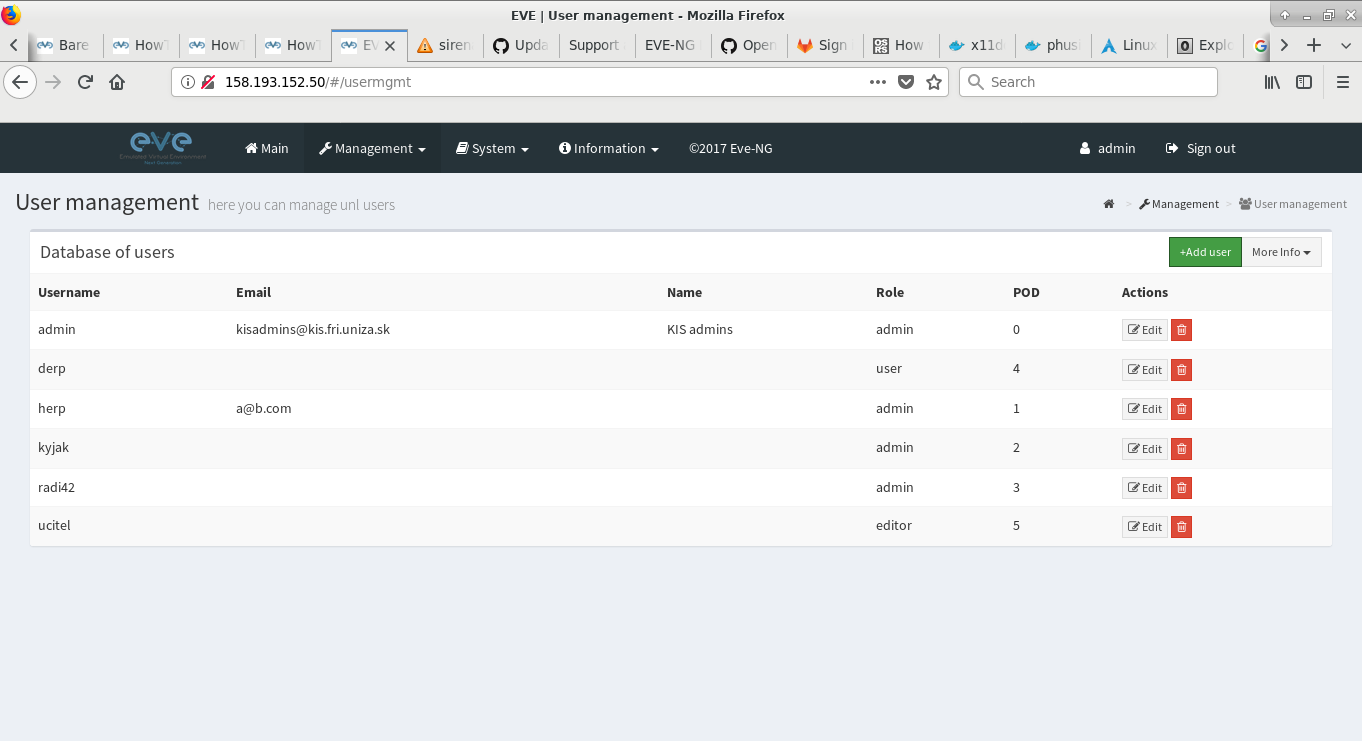
\includegraphics[width=0.75\textwidth]{eve_ng_pouzivatelia_web}
    \caption{Zoznam používateľov vo webovom rozhraní EVE-ng}
    \label{obr:eve_ng_pouzivatelia_web}
\end{figure}

Významom používateľských rolí v EVE-ng sa budeme zaoberať v kapitole \ref{chap:nasadenie_do_vyucovania} - \nameref{chap:nasadenie_do_vyucovania}.




\subsection{Úprava používateľských atribútov}

Atribúty jednotlivých používateľov je možné meniť na obrazovke \emph{User mangement} a môže ich meniť iba používateľ s administrátorskými oprávneniami. Niektoré atribúty, ako sú napr. celé meno používateľa alebo email, sa síce dajú nastaviť, ale následne sa nedajú odstrániť t.j. nastaviť na prázdnu hodnotu. Zmeny sa neprejavia ani vo web rozhraní v zozname používateľov (obrázok \ref{obr:eve_ng_pouzivatelia_web_email_predtym}), ani v MySQL databáze.

\begin{figure}
    \centering
    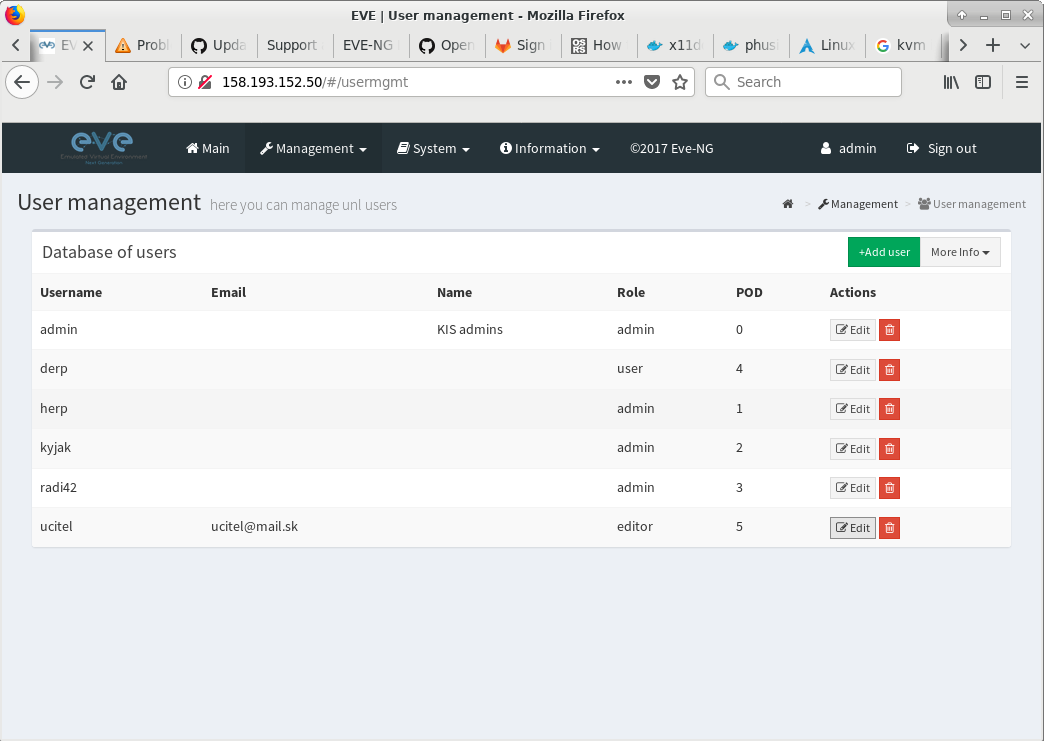
\includegraphics[width=0.75\textwidth]{eve_ng_pouzivatelia_web_email_predtym}
    \caption{Stav pred odstránením e-mail atribútu používateľa \emph{ucitel}}
    \label{obr:eve_ng_pouzivatelia_web_email_predtym}
\end{figure}

Skúsili sme teda odchytiť komunikáciu pri upravovaní spomenutých používateľských atribútov. Zistili sme, po úprave používateľa sa posiela správa \texttt{User saved (60042)} (obrázok \ref{obr:eve_ng_60042}).

\begin{figure}
    \centering
    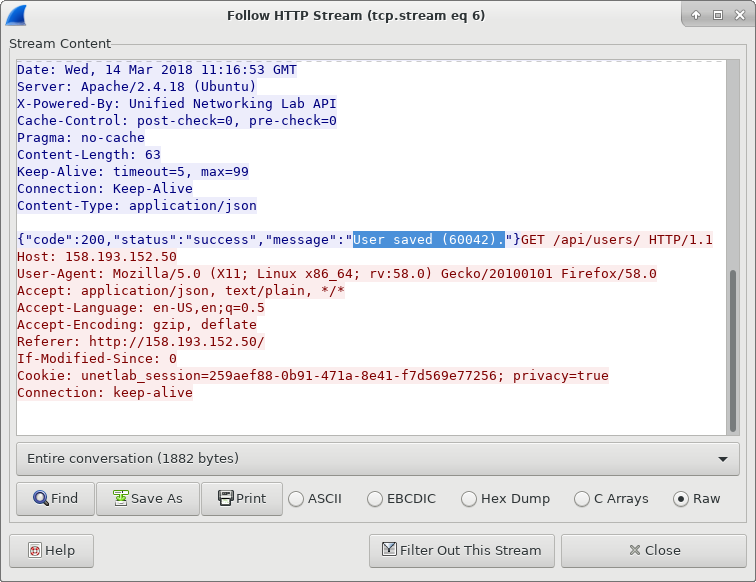
\includegraphics[width=0.75\textwidth]{eve_ng_60042}
    \caption{Správa 60042 - úspešné uloženie atribútov pre používateľa}
    \label{obr:eve_ng_60042}
\end{figure}

Nástroj \emph{grep} ukázal, že kód správy sa vyskytoval o.i. aj v súbore \\
\texttt{/opt/unetlab/html/includes/api\_uusers.php}, konkrétne aj vo funkcii \texttt{apiEditUUser}. Tá ziskava informácie o používateľovi z webového formulára pri úprave tohto používateľa a kontroluje ich správny formát. V prípade, že informácie zadané do webového formulára sú platné, aktualizujú sa atribúty pre konkrétneho používateľa v databáze, v opačnom prípade sa chybne zadané atribúty preskočia.

Problém bol v kontrole vstupov z webového formulára pri úprave používateľa, ktoré boli príliš striktné t.j. nedovoľovali zadať prázdnu hodnotu.

Riešenie spočívalo v upravení kritérii pre atrubúty tak, aby bol aj prázdny reťazec platnou hodnotou.

Po úprave sa už dalo používateľom nielen nastaviť ich celé meno či email, ale aj spomenuté atribúty odstrániť (obrázok \ref{obr:eve_ng_pouzivatelia_web_email_potom}).

\begin{figure}
    \centering
    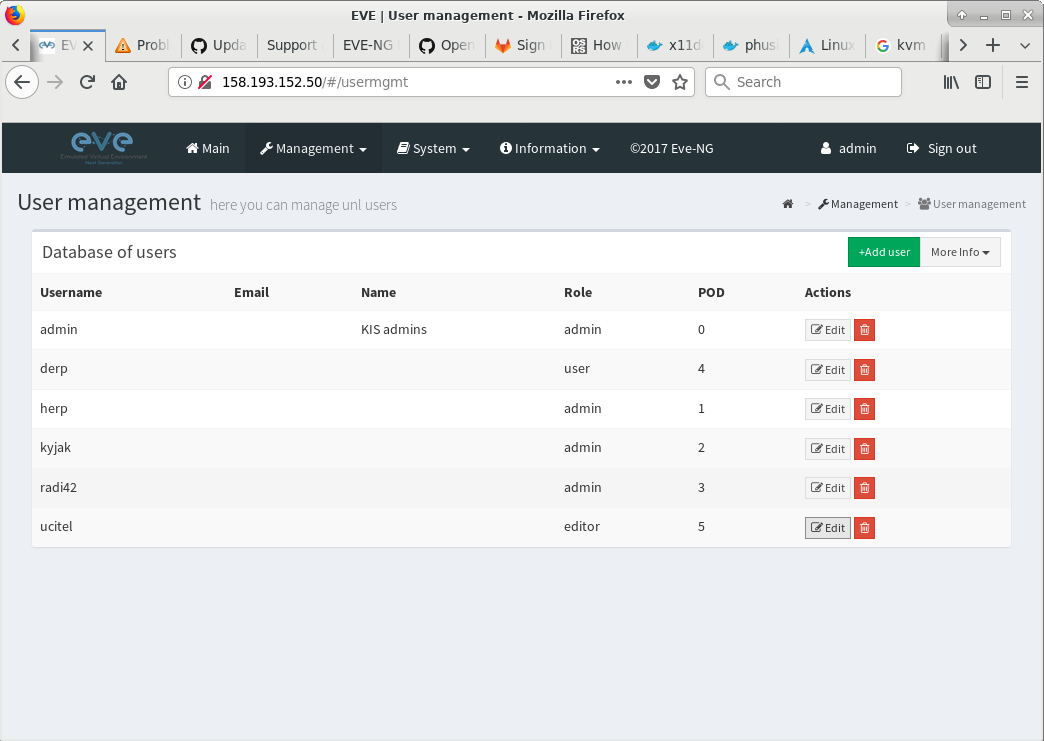
\includegraphics[width=0.75\textwidth]{eve_ng_pouzivatelia_web_email_potom}
    \caption{Zoznam používateľov po odstránení e-mail atribútu pre používateľa \emph{ucitel}}
    \label{obr:eve_ng_pouzivatelia_web_email_potom}
\end{figure}




\subsection{Vypnutie správy o nízkom rozlíšení obrazovky}

Po zmenšení šírky okna približne pod 992 pixelov sa zobrazila správa \\
\texttt{Display too small. This device is not large enough, you need 992px width at least.} (obrázok \ref{obr:eve_ng_display_too_small}).

\begin{figure}
    \centering
    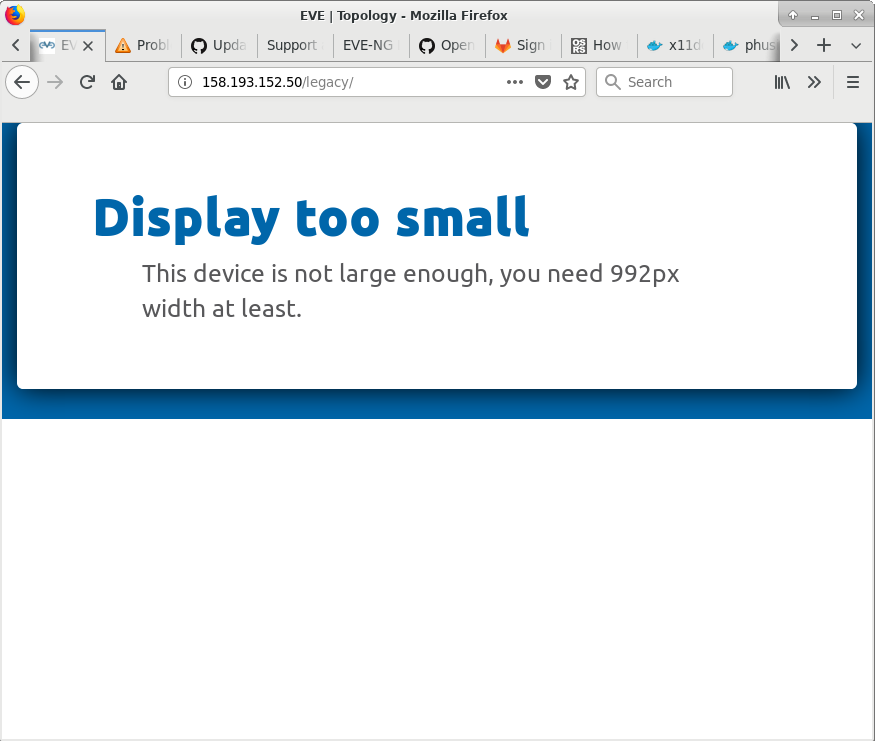
\includegraphics[width=0.75\textwidth]{eve_ng_display_too_small}
    \caption{Chybová správa - \texttt{Display too small.}}
    \label{obr:eve_ng_display_too_small}
\end{figure}

Preto som začal príkazom \emph{grep} hľadať súbory, obsahujúce časti tejto správy. Výstup príkazu obsahoval súbor \\ \texttt{/opt/unetlab/html/themes/default/index.html} \\
ktorý ako jediný obsahoval tento text v nižšie uvedenej časti kódu.

\begin{verbatim}
...
<body>
        <div class="hidden-md hidden-lg container" id="small">
                ...
        </div>
        <div class="hidden-xs hidden-sm container-fluid" id="body">
                ...
        </div>
</body>
...
\end{verbatim}

Skúsili sme zakomentovať všetky riadky v sekcii \texttt{body}, ale následkom tejto zmeny sa stalo otváranie topológii nestabilné a vyskytovali sa rôzne grafické chyby vo vykresľovaní topológie a jej prvkov.

Po experimentovaní so zakomentovaním a upravovaním rôznych riadkov sme našli spôsob, ako túto správu vypnúť. Riešenie spočívalo v zakomentovaní celej sekcie \texttt{div} obsahujúcu atribút \texttt{id="small"} a odstránení tried \texttt{hidden-xs} a \texttt{hidden-sm} z definície sekcie \texttt{div} s atribútom \texttt{id="body"}.

\begin{verbatim}
...
<body>
        <!--<div class="hidden-md hidden-lg container" id="small">
                ...
        </div>-->
        <!--<div class="hidden-xs hidden-sm container-fluid" id="body">-->
        <div class="container-fluid" id="body">
</body>
...
\end{verbatim}

Prvá úprava vypne hlásenie o nízkom rozlíšení obrazovky. Po uložení súboru po prvej úprave a znovunačítaní stránky uvidíme prazdnu bielu obrazovku, ak je okno prehliadača príliš malé t.j. menšie ako približne 992 pixelov.

Druhá úprava odstráni obmedzenie pri vykresľovaní obsahu topológie. Po uložení súboru po prvej úprave a znovunačítaní stránky uvidíme pôvodnú topológiu bez výrazných grafických chýb aj vtedy, ak je okno prehliadača príliš malé t.j. menšie ako približne 992 pixelov.

Po vykonaných úpravách sa problém so zobrazovaním chybovej správy vyriešil, avšak sa vyskytol jeden kozmetický nedostatok. Po zmenšení okna sa zdeformoval posuvník na približovanie a odďaľovanie topológie po zmenšení okna pod kritickú hranicu približne 992 pixelov (obrázok \ref{obr:eve_ng_display_too_small_fixed_but_zoomslider_deformed}).

\begin{figure}
    \centering
    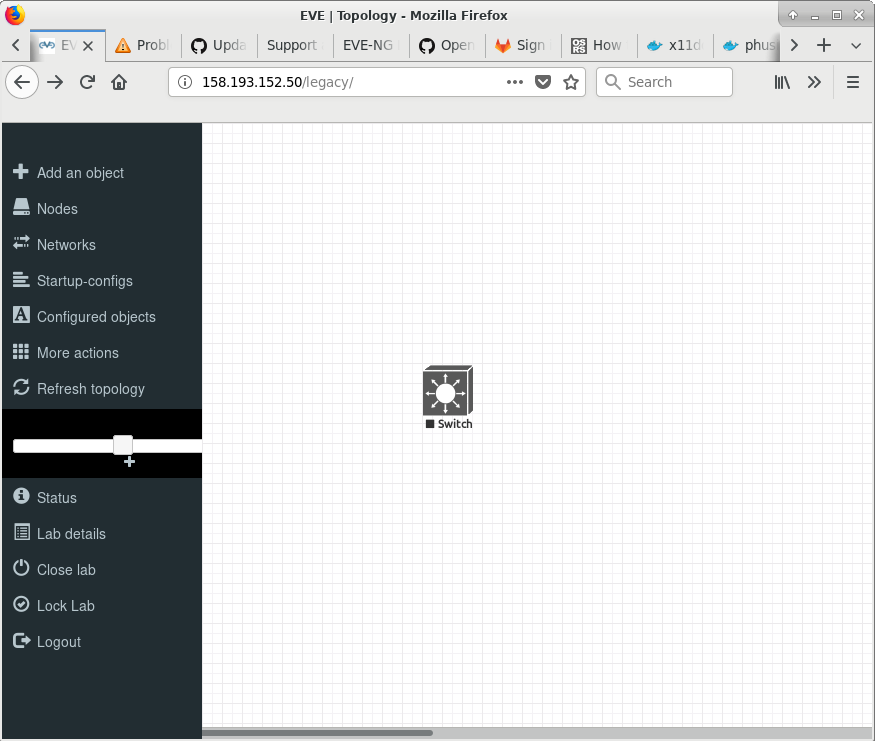
\includegraphics[width=0.75\textwidth]{eve_ng_display_too_small_fixed_but_zoomslider_deformed}
    \caption{Vyriešenie problému s chybovým hlásením \texttt{Display too small.} a deformácia posuvníku na približovanie a odďaľovanie topológie}
    \label{obr:eve_ng_display_too_small_fixed_but_zoomslider_deformed}
\end{figure}

Tento problém sa nám nepodarilo ošetriť. Z "Inšpektora prvkov" vo webovom prehliadači sme zistili, že tento jav môžu spôsobovať napevno zadané hodnoty v súboroch
\begin{verbatim}
/opt/unetlab/html/themes/default/bootstrap/css/bootstrap.min.css
/opt/unetlab/html/themes/adminLTE/build/bootstrap-less/variables.less
\end{verbatim}

Samotný prvok sa volá \texttt{plus-minus-slider} a posuvná plocha sa volá \texttt{zoomslide}, Preto sa riešenie môže skrývať v úprave súborov z výstupu príkazov
\begin{verbatim}
grep -rnw '/opt/unetlab/html/' -e 'plus-minus-slider'
grep -rnw '/opt/unetlab/html/' -e 'zoomslide'
\end{verbatim}

Bol to práve prvok \texttt{zoomslide}, ktorý sa neúmerne zväčšil. Jeho funkčnosť - približovať a oddaľovať prvky v topológii však zostala zachovaná aj napriek tomuto vedľajšiemu účinku.




\subsection{Zatvorenie topológie so spustenými zariadeniami}

Topológiu sa nepodarí zatvoriť, pokiaľ obsahuje spustené zariadenia. Pri zatvorení topológie so spustenými zariadeniami sa vypíše chybové hlásenie \\
\texttt{There are running nodes, you need to power off them before closing the lab.} (obrázok \ref{obr:eve_ng_running_nodes}). \\

\begin{figure}
    \centering
    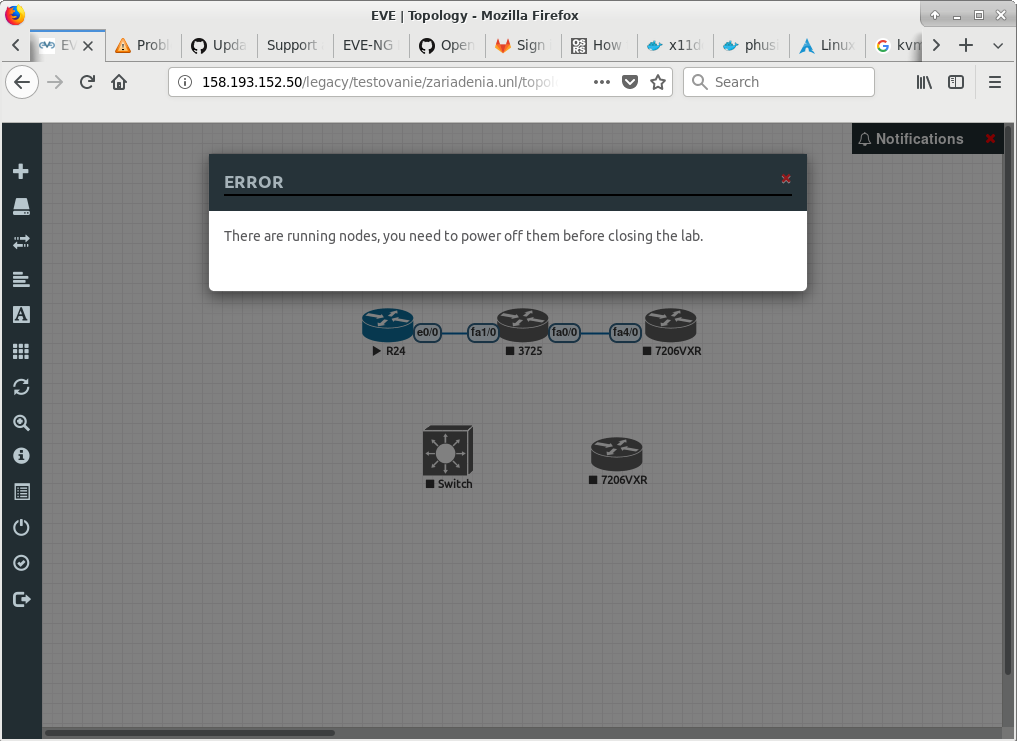
\includegraphics[width=0.75\textwidth]{eve_ng_running_nodes}
    \caption{Chybové hlásenie - topológia so spustenými zariadeniami sa nedá zatvoriť}
    \label{obr:eve_ng_running_nodes}
\end{figure}

Preto sme nástrojom \emph{grep} hľadali, v ktorých súboroch sa vyskytujú časti tejto chybovej správy. Výstup príkazu ukazoval na nižšie uvedené súbory. \\
\begin{verbatim}
/opt/unetlab/html/themes/adminLTE/unl_data/js/angularjs/controllers/lab/labCtrl.js
/opt/unetlab/html/themes/default/js/messages_en.js
\end{verbatim}

Keďže v súbore \texttt{messages\_en.js} sa vyskytujú iba definície chybových hlásení, rozhodoli sme sa upravovať súbor \texttt{labCtrl.js}. V súbore
\begin{verbatim}
/opt/unetlab/html/themes/adminLTE/unl_data/js/angularjs/controllers/lab/labCtrl.js
\end{verbatim}
sa síce táto správa vyskytuje, ale zakomentovanie ľubovoľnej relevantnej časti kódu v metóde \texttt{closeLab} nemá vplyv na funkčnosť t.j. chybové hlásenie sa pri zatvorení topológie napriek tomu zobrazí.

Preto sme sa nakoniec pozreli do súboru \texttt{messages\_en.js}. V ňom bola chybová správa definovaná v poli \texttt{MESSAGES} ako \texttt{MESSAGES[131]}. Znova sa začalo hľadanie výskytov tohto reťazca v súboroch nástrojom \emph{grep}. Výstup príkazu ukazoval na súbory
\begin{verbatim}
/opt/unetlab/html/themes/default/js/functions.js
/opt/unetlab/html/themes/default/js/messages_en.js
\end{verbatim}

Keďže súborom \texttt{messages\_en.js} sme sa už zaoberali, pokračoval som súborom \texttt{functions.js}. V ňom sa vyskytovala aj funkcia \texttt{closeLab}. Tá obsahovala nielen chybové hlásenie, ale aj kontrolu, či v topológii sú už spustené zariadenia. Vypli sme teda túto kontrolu zakomentovaním riadku s podmienkou "if" a celej vetvy "else", ako je uvedené nižšie.
\begin{verbatim}
        //if (running_nodes == false) {
            ...
        //} else {
        //    deferred.reject(MESSAGES[131]);
        //}
\end{verbatim}

Potom sme sa odhlásili, vymazali vyrovnávaciu pamäť webového prehliadača a prihlásili sa do EVE-ng ako používateľ s rolou \texttt{admin}. Potom sme si otvorili súbor s topológiou a pridali do nej niekoľko zariadení. Spustili som zariadenie a pokúsil sa zatvoriť topológiu. Teraz sa chybové hlásenie nezobrazilo a topológia sa úspešne zatvorila. Po znovuotvorení rovnakej topológie zostali zariadenia spustené. Bolo možné aj spustiť ďalšie zariadenia.

Keď sme sa ešte predtým rozhodli riešiť problém so zatváraním topológie so spustenými zariadeniami, skúšali sme v súbore \texttt{functions.js} vo funkcii \texttt{closeLab} zakomentovať celý \texttt{for} cyklus v riadku 
\begin{verbatim}
    $.each(values, function (node_id, node) {
        if (node['status'] > 1) {
            running_nodes = true;
        }
    });
\end{verbatim}
keďže aj v ňom sa nastavovala premenná \texttt{running\_nodes} Po zakomentovaní cyklu sa topológia síce dala zatvoriť aj pri spustených zariadeniach, ale so zariadeniami v nej sa nedalo pracovať napr. nebolo možné zastaviť už spustené zariadenia alebo spustiť ďalšie.

Po opravení tohto nedostatku sa ale vyskytol ďalší problém, ktorý sa odhalil až po vyriešení momentálneho, a síce, že po zatvorení jednej topológie (obrázok \ref{obr:eve_ng_zle_portove_cisla_1}) a otvorení inej (obrázok \ref{obr:eve_ng_zle_portove_cisla_2}) sa zariadenia tvárili, že sú spustené, hoci predtým spustené neboli. Obidva obrázky ukazujú rovnaký počet spustených zariadení v dvoch rôznych topológiách, pričom zariadenia boli spustené iba v topológii na obrázku \ref{obr:eve_ng_zle_portove_cisla_1}. Zariadenia v iných topológiách mali znefunkčnený vzdialený prístup a nešlo s nimi pracovať. Správne fungovali iba tie v pôvodnej topológii. Pokiaľ mali topológie rovnaký počet zariadení a do druhej sme pridali nové zariadenie, toto zariadenie fungovalo bez komplikácii.

Tento jav nastal kvôli tomu, že portové čísla pre jednotlivé zariadenia v topológii sa začínajú číslovať od začiatku rozsahu, ktorý je pridelený danému používateľovi, bez ohľadu na to, ktorá topológia je momentálne otvorená.

Spomenutý problém s rovnakými portovými číslami pre zariadenia v rôznych topológiách sa nám nepodarilo vyriešiť, pretože sa jedná o hlbší problém, ktorého riešenie by znamenalo zmenu mechanizmu na prideľovanie portových čísel v EVE-ng.

\begin{figure}
    \centering
    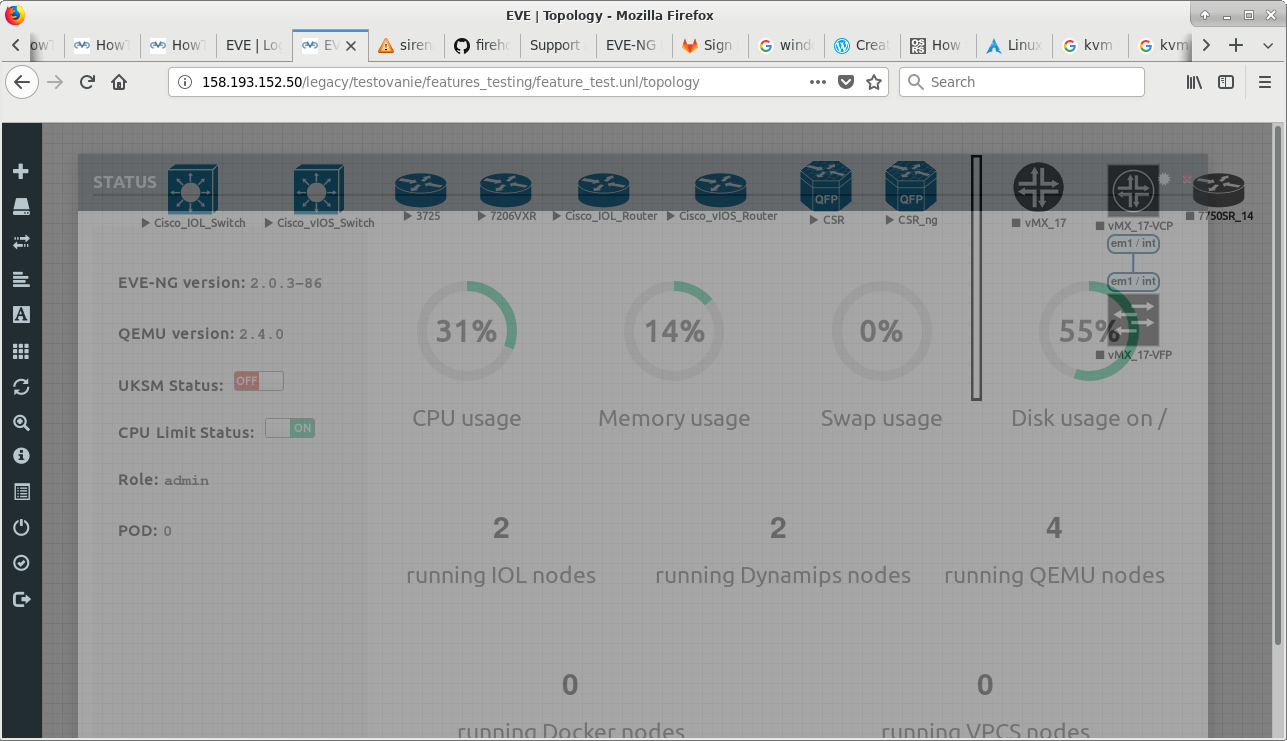
\includegraphics[width=0.75\textwidth]{eve_ng_zle_portove_cisla_1}
    \caption{Prvá topológia a celkový počet spustených zariadení}
    \label{obr:eve_ng_zle_portove_cisla_1}
\end{figure}

\begin{figure}
    \centering
    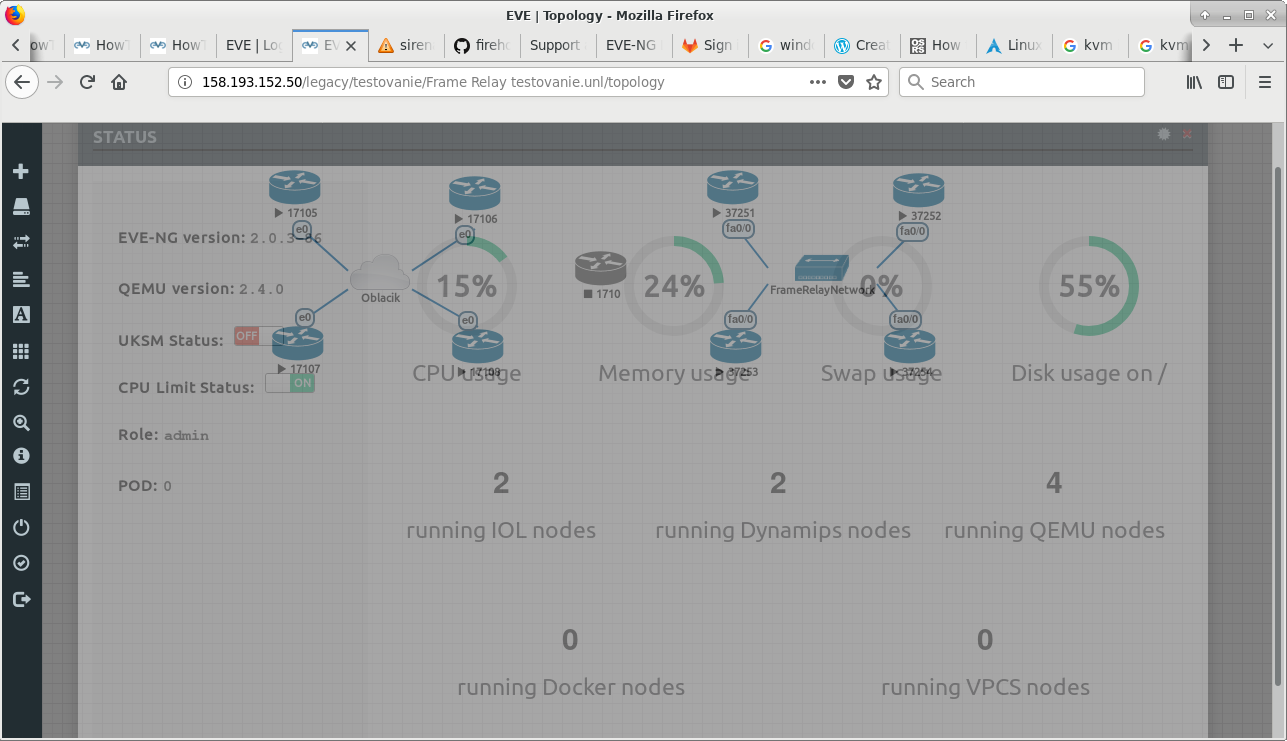
\includegraphics[width=0.75\textwidth]{eve_ng_zle_portove_cisla_2}
    \caption{Druhá topológia a celkový počet spustených zariadení}
    \label{obr:eve_ng_zle_portove_cisla_2}
\end{figure}

Komplikácie, na ktoré sme narazili počas nasadenia na predmety, sú popísané v kapitole \ref{chap:nasadenie_do_vyucovania} - \nameref{chap:nasadenie_do_vyucovania}.




\section{Administrácia}

EVE-ng server je vytvorený tak, aby sa po jeho konfigurácii bolo potrebné oň starať čo najmenej. V nasledujúcich častiach budú opísané veci súvisiace s jeho administráciou.




\subsection{Adresárova štruktúra}
\label{chap:adresarova_struktura}

Tu je uvedený krátky zoznam najdôležitejších adresárov v EVE-ng. Podrobnejší zoznam súborov a adresárov sa nachádza v dokumentácii na priloženom CD.

\begin{longtabu} to \textwidth {| X[3.0,l,m] | X[4.0,l,m] |}
\caption{Adresárová štrukúra EVE-ng servera}
\label{tab:adresare} \\
\hline
    \multicolumn{1}{|c|}{\textbf{Adresár}} & \multicolumn{1}{|c|}{\textbf{Popis}} \\
\hline
    \texttt{/opt/unetlab/addons/} & \makecell[lc]{Adresár obsahujúci všetky zariadenia, \\ ktoré je možné pridať do topológie. \\ Obsahuje podadresáre \texttt{dynamips}, \texttt{iol} a \texttt{qemu}, \\ podľa toho, pre aký typ hypervízora je zariadenie \\ určené - Dynamips, IOL alebo QEMU/KVM} \\
\hline
    \texttt{/opt/unetlab/addons/iol/bin/} & \makecell[lc]{Adresár s Cisco IOL zariadeniami spolu s \\ vygenerovanou IOL licenciou} \\
\hline
    \texttt{/opt/unetlab/addons/iol/lib/} & \makecell[lc]{Adresár s Cisco IOL ovládačom potrebným \\ na spustenie Cisco IOL zariadenia} \\
\hline
    \texttt{/opt/unetlab/html/templates/} & Šablóny pre každý typ zariadenia v topológii \\
\hline
    \texttt{/opt/unetlab/data/Logs} & Súbory o zázname činností na serveri \\
\hline
\end{longtabu}




\subsection{Zálohovanie}
\label{chap:zalohovanie}

Kritické súbory a adresáre sú automatizovane zálohované nástrojmi \emph{cron} a \emph{rsync}. Pre tento účel bol vytvorený skript, ktorý používa nástroj \emph{rsync}. Ten synchronizuje adresáre a súbory len vtedy, pokiaľ zistí, že sa majú nahradiť novšími verziami. Nástroj \emph{cron} je nastavený tak, že vykonáva tento skript každý deň počas noci, kedy sa na serveri vyskytuje minimálna aktivita.




\subsection{Monitorovanie}

Monitorovanie systému je dôležitým prostriedkom v prípade, že zaznamenáme nižšiu výkonnosť servera. Na monitorovanie systémových zdrojov EVE-ng servera môžeme, okrem tradičného nástroja \emph{htop} použiť aj vstavaný nástroj na monitorovanie systémových zdrojov vo webovom rozhraní EVE-ng.

Vstavaný monitorovací systém EVE-ng sa nachádza vo webovom rozhraní v časti \emph{System} -> \emph{System status}. Rovnaký panel je prístupný aj z rozhrania topológie v menu na ľavej strane obrazovky po kliknutí na položku \emph{Status}. Zobrazuje prehľad o aktuálnom percentuálnom vyťažení procesora, operačnej pamäte a diskového priestoru spolu s celkovým počtom spustených zariadení každého druhu. Nástroj je znázornený na obrázku \ref{obr:eve_ng_system_status}.

\begin{figure}
    \centering
    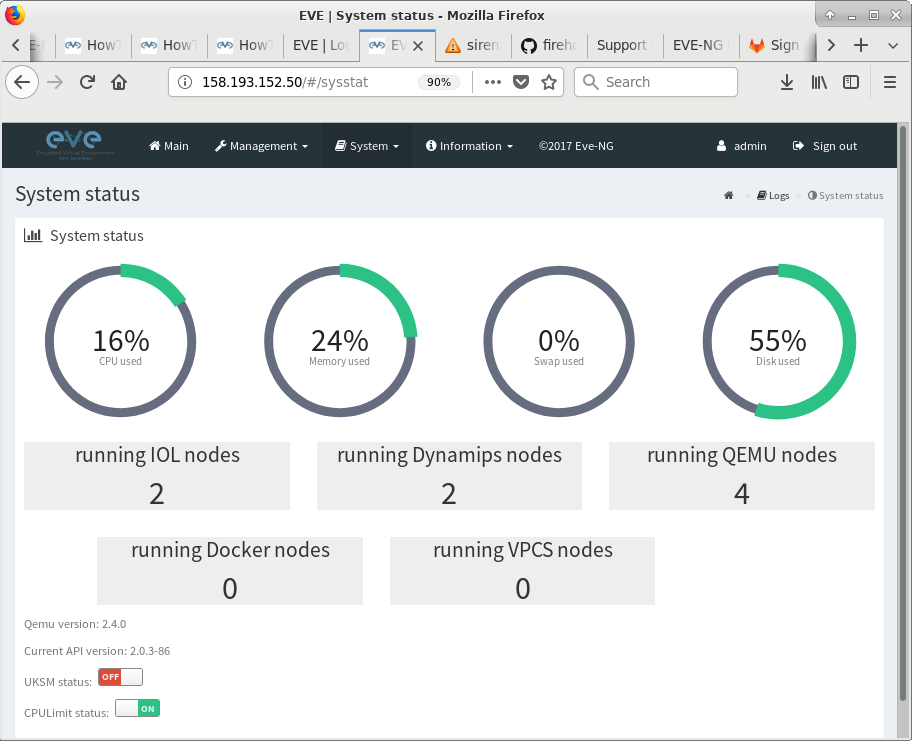
\includegraphics[width=0.75\textwidth]{eve_ng_system_status}
    \caption{Monitorovanie systému vo webovom rozhraní EVE-ng}
    \label{obr:eve_ng_system_status}
\end{figure}




\subsection{Správa používateľov EVE-ng}

Zoznam používateľov webového rozhrania v EVE-ng je znázornený na obrázku \ref{obr:eve_ng_pouzivatelia_web_email_potom} (str. \pageref{obr:eve_ng_pouzivatelia_web_email_potom}). Obrazovka sa nazýva \emph{User management} a je prístupná z horného menu kliknutím na \emph{Management} -> \emph{User management}. Pre každého používateľa sú definované nasledujúce stĺpce:

\begin{itemize}[noitemsep]
    \item \textbf{Username} - Používateľské meno. Používa sa na prihlásenie sa do webového rozhrania. Musí byť unikátne pre každého používateľa.
    \item \textbf{Email} - Emailová adresa.
    \item \textbf{Name} - Celé meno používateľa. Atribút má iba informatívny charakter.
    \item \textbf{Role} - Používateľská rola. Definuje oprávnenia prihláseného používateľa.
    \item \textbf{POD} - Identifikačné číslo používateľa. Určuje rozsah portov, ktoré sa používajú na vzdialený prístup ku zariadeniam v topológii. Musí byť unikátne pre každého používateľa.
    \item \textbf{Actions} - Úprava atribútov používateľa (Edit) a odstránenie používateľa (Delete). Po kliknutí na tlačidlo \emph{Edit} v riadku vybraného používateľa sa otvorí dialógové okno na vytvorenie a úpravu používateľa zobrazené na obrázku \ref{obr:eve_ng_pouzivatelia_dialog} (str. \pageref{obr:eve_ng_pouzivatelia_dialog}).
\end{itemize}

Dialógové okno na vytvorenie a úpravu používateľa sa zobrazí po kliknutí na tlačidlá \emph{Add user} a \emph{Edit}. Pozostáva z týchto častí:

\begin{itemize}[noitemsep]
    \item User Name
    \item Password
    \item Password Confirmation
    \item Email
    \item Name
    \item Role
    \item POD
\end{itemize}

Všetky polia majú rovnaký význam ako v popise stĺpcov na obrazovke so zoznamom používateľov. Novým prvkom sú polia \emph{Password} a \emph{Password Confirmation}. Tie nie je nutné vypĺňať, ak ich nechceme meniť. Ak chceme používateľovi heslo zmeniť, je potrebné zadať nové heslo do obidvoch polí. Na zmenu hesla na nové nie je nutné zadávať pôvodné heslo. Pole \emph{User Name} sa pri úprave používateľa nedá zmeniť, dá sa iba jednorázovo nastaviť pri vytváraní používateľa. Pole \emph{POD} je vyplnené automaticky najnižším voľným identifikátorom.

Ak sme vykonali kroky v časti \ref{chap:eve_ng_pouzivatelske_role} - \nameref{chap:eve_ng_pouzivatelske_role}, budú po kliknutí na rozbaľovací zoznam pre atribút \emph{Role} dostupné, okrem role \emph{admin}, aj role \emph{editor} a \emph{user}. Tieto role sa medzi sebou líšia oprávneniami na výkon určitých činností. Zoznam činností pre každú používateľskú rolu je popísaný v nižšie uvedených zoznamoch.

\noindent
Zoznam úloh, ktoré môže vykonávať používateľ s rolou \emph{user}:

\begin{itemize}[noitemsep]
    \item Prehliadať súbory a adresáre
    \item Prehliadať topológiu
\end{itemize}

\noindent
Zoznam úloh, ktoré môže vykonávať používateľ s rolou \emph{editor}:

\begin{itemize}[noitemsep]
    \item Všetko, čo môže vykonávať používateľ s rolou \emph{user}
    \item Spravovať súbory a adresáre - vytváranie, presúvanie, premenovanie, odstránenie
    \item Upravovať prvky v topológii - pridávanie, presúvanie, premenovanie, odstránenie
    \item Upravovať vybrané atribúty používateľov - meno, email
    \item Exportovať/importovať súbory s topológiami
    \item Zamknúť topológiu, aby bola pre používateľov typu \emph{user} iba na čítanie
\end{itemize}

\noindent
Zoznam úloh, ktoré môže vykonávať používateľ s rolou \emph{admin}:

\begin{itemize}[noitemsep]
    \item Všetko, čo môže vykonávať používateľ s rolou "editor"
    \item Zastaviť všetky zariadenia v "System -> Stop All Nodes"
    \item Zobraziť informácie o konkrétnom používateľovi cez API
    \item Spravovať všetkých používateľov - pridať, upraviť, odstrániť
    \item Zapnúť/vypnúť UKSM v "System -> System status"
    \item Zapnúť/vypnúť KSM v "System -> System status", ak je KSM dostupné
    \item Zapnúť/vypnúť CPULimit v "System -> System status"
    \item Aktualizovať EVE-ng z web rozhrania cez koncový bod "/api/update" v UNetLab/EVE-ng API
\end{itemize}

Niektoré z týchto činností nie sú implementované vo webovom rozhraní EVE-ng. Činnosti, ktoré môžu vykonávať jednotlivé používateľské role sú definované v súbore "/opt/unetlab/html/api.php". Vyznačujú ich riadky

\begin{verbatim}
  ...
  if (!in_array($user['role'], Array('admin'))) {
  ...

resp.

  ...
  if (!in_array($user['role'], Array('admin', 'editor'))) {
  ...
\end{verbatim}

Vyššie uvedené podmienky kontrolujú, či je používateľ s danou rolou oprávnený vykonať požadovanú operáciu. Napr. vytvoriť používateľa, premenovať adresár, presunúť súbory do adresára a pod.

V prípade, že používateľ nemá dostatočné oprávnenia sa zobrazí chybové hlásenie \texttt{Not enough access privileges for this operation (90032)}, ktoré znázornené na obrázku \ref{obr:not_enough_access_privileges}.

\begin{figure}
    \centering
    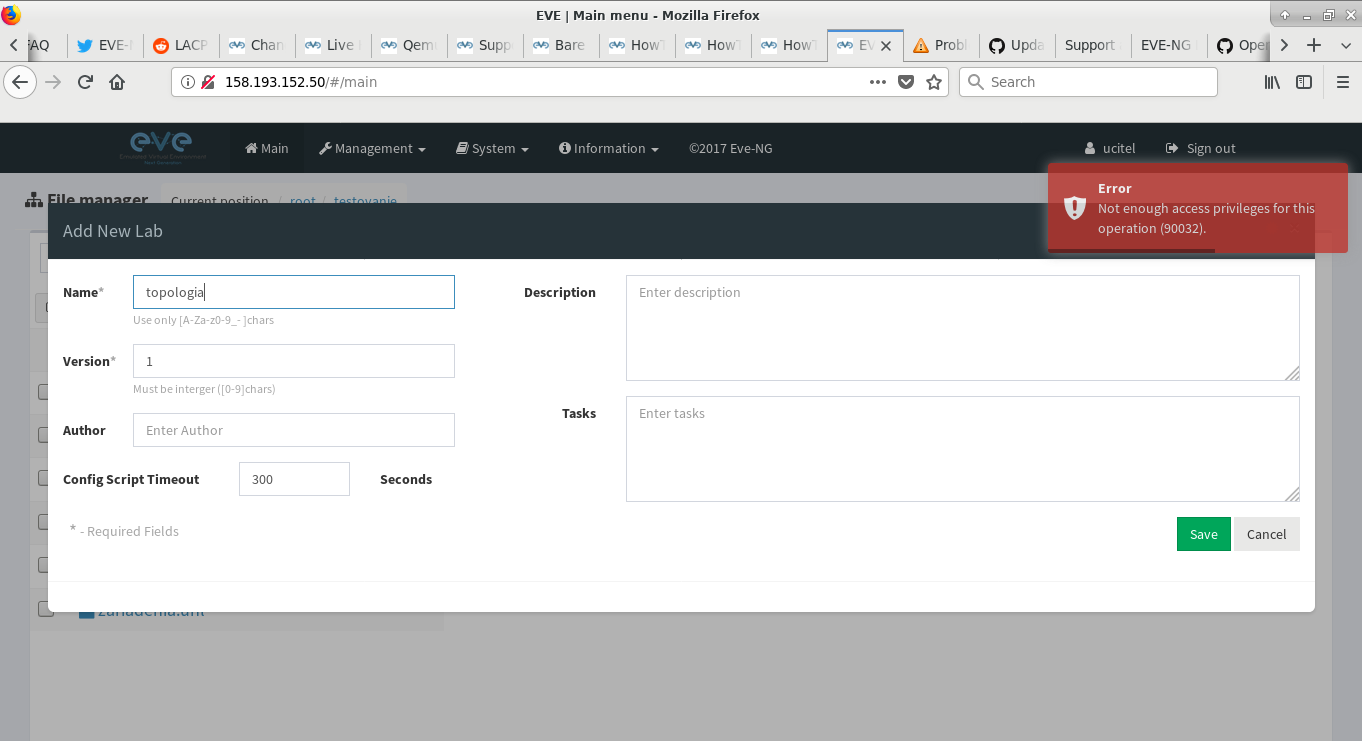
\includegraphics[width=0.75\textwidth]{not_enough_access_privileges}
    \caption{Chybové hlásenie o nedostatočných oprávneniach používateľa}
    \label{obr:not_enough_access_privileges}
\end{figure}

Niekedy sa však táto správa pri vykonaní neoprávnenej činnosti nezobrazí, čo ale nemá žiadny vplyv na funkcionalitu a daná operácia sa nevykoná.
\chapter{Analýza vyučovania}

Aktuálny stav na katedre: aké virtuálne nástroje sa používajú na katedre a v akých predmetoch.

\section{Vybrané predmety}

Ku všetkým predmetom vytvoriť zoznam technológii.

\subsection{Počítačové siete 1}

\subsection{Počítačové siete 2}

\subsection{Projektovanie sietí 1}

\subsection{Projektovanie sietí 2}

\subsection{CCNP Routing}

\subsection{CCNP Switching}
\chapter{Virtuálne zariadenia}
\label{chap:virt_zariadenia}

Dôležitú súčasť virtuálneho laboratória tvoria aj jeho zariadenia. Po analýze vyučovania sme mohli začať s ich získavaním a testovaním.




\section{Získavanie}

Zariadenia boli získavané z rôznych zdrojov. Predovšetkým boli použité zariadenia, ktoré sa už na katedre používali.

Ako už bolo naznačené v časti \ref{chap:adresarova_struktura}, EVE-ng podporuje rôzne typy zariadení. Patria medzi ne zariadenia typu Dynamips, Cisco IOL/IOU a QEMU.

Zoznam všetkých funkčných zariadení v nástroji EVE-ng je k dispozícii na CD médiu.




\subsubsection{Metodika}

Pri získavaní zariadení sme vychádzali zo zariadení, ktoré sa na katedre používajú a zo zoznamu zariadení, ktoré nástroj EVE-ng podporoval. Vybrané zariadenia následne prechádzali testovacími krokmi, ktoré sú bližšie popísané v ďalších častiach tejto kapitoly.

Všetky zozbierané zariadenia sú uložené v adresári \\ \texttt{/opt/unetlab/addons/rozne\_zariadenia}.




\section{Testovanie}
\label{chap:testovanie_zariadeni}

Testovanie zariadení bolo vykonané, aby sa zaistila kvalita a plynulosť vyučovacieho procesu, ako aj predvídateľnosť a replikovateľnosť behu jednotlivých zariadení a topológii.




\subsection{Testovanie spustiteľnosti}

Ako prvé bola testovaná spustiteľnosť zariadení. Na základe nej sa zistilo, či je zariadenie schopné zapnúť a konfigurovať ho pomocou vzdialeného prístupu.



\subsubsection{Metodika}

Najpr bolo potrebné pridať zariadenie na server. Môžeme na to použiť návody buď z oficiálnej EVE-ng stránky \cite{eve_ng_howtos}. Návody pre niektoré zariadenia sú k dispozícii aj na CD v adresári \emph{eve-ng}.

Vybrané zariadenia sme následne pridávali do predpripravenej topológie v EVE-ng. Následne sme vybrali jedno zariadenie, ktoré sme následne spustili. Ak sa zariadenie nespustilo, skúšali sme zistiť príčinu a vykonávali rôzne úpravy, akými by sme zariadenie v topológii spustili napr. modifikovať súbor, z ktorého sa zariadenie spúšťalo, opraviť oprávnenia, premenovať súbor do správneho formátu, upraviť systémové parametre na zariadenia a pod.

Ak sa zariadenie spustilo, skúsili sme sa pripojiť na jeho konzolu. Keď sa na ňu nedalo pripojiť, zariadenie sme zastavili a zmenili protokol na vzdialený prístup; obvykle stačilo vyskúšať protokoly \emph{telnet} a \emph{vnc}. V prípade, že zariadenie je v poriadku, mali by sme aspoň jedným z týchto protokolov dostať textový resp. grafický výstup konzoly na zariadení.

Ak sme sa nakoniec pripojili ku konzole zariadenia, sledovali sme jeho spúšťanie. Čakali sme na dokončenie spúšťania. V prípade, že sa zariadenie úspešne spustilo, prihlásili sme da doň predvolenými prihlasovacími údajmi, ak to bolo potrebné, a vyskúšali sme, či konzola reaguje na vstup z klávesnice. Ak konzola reagovala, zariadenie zostalo uložené na serveri. Ak sme ku zariadeniu nevedeli zistiť prihlasovacie údaje, umiestnili sme ho do osobitného adresára.

Ak sa ani po týchto úkonoch zariadenie nespustilo, odstránili sme ho zo servera. Týmto spôsobom sme získali množinu spustiteľných zariadení v EVE-ng topológii.

\subsubsection{Vyhodnotenie}

Výsledky testovania spustiteľnosti zariadení sú zhrnuté v súbore \\ \emph{sumarny\_prehlad\_podporovanych\_zariadeni\_vo\_virtualnych\_sietovych\_nastrojoch.ods}. Súbor obsahuje viacero stĺpcov, ktorých význam je bližšie vysvetlený v tabuľke \ref{tab:sumarny_prehlad_stlpce}. Z výstupov tohto testovania bol vytvorený aj skript na úpravu šablón, ktorý je bližšie opísaný v závere tejto časti.

\begin{longtabu} to \textwidth {| X[2.5,l,m] | X[5.0,l,m] |}
\caption{Stĺpce v sumárnom prehľade zariadení}
\label{tab:sumarny_prehlad_stlpce} \\
\hline
    \multicolumn{1}{|c|}{\textbf{Stĺpec}} & \multicolumn{1}{|c|}{\textbf{Popis}} \\
\hline
    \textbf{Zariadenie} & \makecell[lc]{Názov alebo modelové označenie zariadenia.} \\
\hline
    \textbf{Platforma} & \makecell[lc]{Názov a verzia operačného systému zariadenia.} \\
\hline
    \textbf{Názov súboru} & \makecell[lc]{Pomenovanie zariadenia na serveri.} \\
\hline
    \textbf{Spôsob virtualizácie} & Hypervízor, pod ktorým zariadenie môže byť spustené. \\
\hline
    \textbf{\makecell[lc]{Predvolené prihlasovacie \\ údaje}} & Predvolené prihlasovacie meno a heslo, ak to zariadenie vyžaduje. \\
\hline
    \textbf{Spôsob pripojenia} & \makecell[lc]{Protokol, ktorý sa používa na vzdialenú konfiguráciu \\ zariadenia.} \\
\hline
    \textbf{Úspešné spustenie} & Informácia, či sa zariadenie v topológii spustilo. \\
\hline
    \textbf{Poznámky} & \makecell[lc]{Bližší popis správania sa daného zariadenia, popr. \\ problémy pri používaní zariadenia a ich možné riešenie. \\ Ďalej sa v ňom môžu nachádzať niektoré podporované \\ technológie a internetové odkazy ako zdroj pre informácie \\ uvádzané pre dané zariadenie.} \\
\hline
\end{longtabu}

Ďalšie stĺpce slúžia pre prieskum spustiteľnosti zariadení v rôznych nástrojoch nasadených na rôznych platformách.

Pokiaľ sme zistili, že protokol vzdialeného prístupu sa odlišuje od predvoleného protokolu v šablóne na EVE-ng serveri, túto šablónu sme museli upraviť ručne. Avšak s postupným nárastom testovaných zariadení rástol aj počet úprav v šablónach pre jednotlivé zariadenia. Preto sme sa rozhodli vytvoriť skript, ktorý by celý proces automatizoval. Tento skript na úpravu šablón upravuje jednotlivé atribúty konkrétnym zariadeniam. Výsledky testovania sa prejavili v skripte na úpravu šablón, v ktorom  boli nastavené atribúty pre protokol na vzdialený prístup k zariadeniam a počte a type rozširujúcich kariet pre zariadenia.




\subsection{Testovanie systémových požiadaviek}
\label{chap:testovanie_zariadeni_benchmark}

Čo som meral?
Prečo som to meral?
Čím som meral?
Čo je výstupom?
Ako som výstup vyhodnotil?

Testovanie systémových požiadaviek zariadení bolo realizované na fyzickom EVE-ng serveri. Tento druh testovania bol dôležitý preto, aby sme mohli danému zariadeniu nastaviť dostatočné technické parametre, čím zaistíme jeho plynulý chod a predídeme rôznym komplikáciám počas používania vo vyučovaní. Tieto parametre sú uložené v šablóne pre dané zariadenie.

Úprava šablón je realizovaná skriptom, po ktorého vykonaní sa príslušným zariadeniam zmenia konkrétne technické parametre v šablóne. Po úprave šablón sa zmeny prejavia okamžite a po pridaní zariadenia do topológie, kedy sa jeho parametre automaticky nastavia na správne hodnoty. Pre vybrané zariadenia boli merané tieto veličiny:

\begin{itemize}
\item Vyťaženie procesora
\item Využitie operačnej pamäte
\item Vyťaženie pevného disku
\end{itemize}

Vyťaženie procesora bolo merané z dôvodu jeho intenzívnej činnosti hlavne počas spúšťania zariadení, ale môže byť vyťažovaný aj po dokončení spúšťania. Na základe toho budeme vedieť určiť, koľko zariadení budeme môcť v topológii spustiť naraz, a koľko už spustených zariadení zvládne server spravovať celkovo. Pri meraní vyťaženia procesora bolo merané celkové vyťaženie aj vyťaženie jednotlivých jadier procesora.

Operačná pamäť je najviac využitá po dokončení spúšťania zariadenia. Kapacita operačnej pamäte ovplyvňuje celkový počet spustených zariadení na serveri. Meranie jej vyťaženia je pomerne jednoduché pre celý systém, ale pre tieto účely sme potrebovali s vysokou presnosťou vedieť, do akej koľko operačnej pamäte využíva iba konkrétne zariadenie.

Na meranie využitia operačnej pamäte boli použité dva nástroje: \texttt{ps} a \texttt{ps\_mem}. Prvý z nich už bol na EVE-ng serveri prítomný, druhý bolo potrebné nainštalovať dodatočne. Na meranie boli použité dva nástroje, aby sa navzájom výsledky oboch nástrojov medzi sebou validovali.

Disk najviac vyťažený predovšetkým pri spúšťaní zariadenia, ale môže byť vyťažený aj po dokončení spúšťania. Vyťaženie disku bolo do merania zahrnuté, aby sme vedeli odhadnúť, do akej miery je spúšťanie a beh zariadení ovplyvnený rýchlosťou pevného disku a o koľko by sa teoreticky zvýšil výkon servera pri ich výmene za SSD disky.

Z merania boli vynechané meranie frekvencie procesora a vyťaženie sieťového rozhrania. Frekvencia procesora bola vynechaná, lebo procesor podľa príkazu \texttt{watch lscpu | grep "MHz"} striedal iba dve frekvencie: 2000.000 MHz (minimálna frekvencia) a 2333.000 MHz (maximálna frekvencia).

Vyťaženie sieťovej karty je zanedbateľné pri meraní výkonnosti jednotlivých zariadení, keďže sa sieť využíva iba na interakciu používateľa s klientskou aplikáciou, čo vytvára zanedbateľnú záťaž.

Na monitorovanie vybraných veličín sú určené rôzne nástroje a stratégie. Mohli sme napr. vytvoriť skript, ktorý by pomocou viacerých špecializovaných nástrojov meral vyťaženie jednotlivých prvkov systému, alebo použiť nástroj, ktorý je schopný monitorovať široké spektrum systémových zdrojov. Zvažovali sme tieto nástroje:

\begin{itemize}
    \item \textbf{iotop} ~~~~~ - ~~monitorovanie procesov podľa využitia disku
    \item \textbf{nmap} ~~~~ - ~~monitorovanie sieťovej prevádzky
    \item \textbf{nethogs} ~ - ~~monitorovanie procesov podľa využitia sieťového rozhrania
    \item \textbf{dstat} ~~~~~~ - ~~monitorovanie rôznych systémových prostriedkov
    \item \textbf{sysstat} ~~~~- ~~monitorovanie rôznych systémových prostriedkov
    \item \textbf{netdata} ~~~- ~~monitorovanie rôznych systémových prostriedkov cez web rozhranie
\end{itemize}

Z uvedených nástrojov sme sa rozhodli použiť nástroj \emph{dstat}. Hlavným dôvodom, prečo sme si sme sa rozhodli ďalej používať a upravovať tento nástroj a uprednostniť ho pred ostatnými nástrojmi, bola možnosť ovládania cez príkazový riadok a ukladanie ziskaných údajov do CSV súboru. Dáta sa do CSV súboru zapisovali každú sekundu. Následne sme si vytvorili tabuľkový dokument, ktorý vyhodnocoval namerané dáta z CSV súboru. Vyhodnocovaním nameraných údajov sa budeme bližšie zaoberať v časti \ref{chap:testovanie_zariadeni_benchmark_vyhodnotenie}.

Nástroj \emph{dstat} však bolo potrebné upraviť tak, aby zisťoval využitie operačnej pamäte iba pre zariadenia v EVE-ng topológii, nie celého systému.

Pre tento účel sme vytvorili kópiu nástroja \emph{dstat} s názvom \emph{dstat\_custom}. V tejto kópii sme následne upravovali jeho zdrojový kód pre naše potreby. Nástroj je vytvorený v programovacom jazyku Python.

Nástroj \emph{dstat\_custom} bol upravený tak, že sa meria využitie operačnej pamäte pre zariadenie v EVE-ng topológii nástrojmi \emph{ps} a \emph{ps\_mem}. Obidva príkazy merajú tú istú množinu procesov patriacich spusteným zariadeniam v EVE-ng topológii, aby sme mohli merania jednotlivých nástrojov medzi sebou porovnať. Hodnoty namerané obomi nástrojmi by mali byť približne rovnaké na to, aby sme mohli výsledky považovať za validné.

Vo výslednom CSV súbore vytvorenom nástrojom \emph{dstat\_custom} sa stĺpce \emph{used} a \emph{buffered} v časti \emph{memory usage} nahradia stĺpcami \emph{MemUsed-ps} a \emph{MemUsed-ps\_mem}.

Aby nástroj \emph{dstat\_custom} fungoval správne, musia byť nainštalované balíčky \emph{dstat}, \emph{ps\_mem} a \emph{sultan}. Význam prvých dvoch balíčkov už bol v tejto časti vysvetlený. Balíček \emph{sultan} slúžil na vykonávanie terminálových príkazov zvnútra Python programu.

Už upravený nástroj \emph{dstat\_custom} je možné nájsť na zálohovacom serveri v adresári \emph{eve\_ng\_specific/usr\_bin/dstat\_custom}.





\subsubsection{Metodika}

Čo bolo potrebné vykonať pred meraním?
Ako prebiehalo meranie?
Čo je výstupom merania?


Testované skriptom - upravený nástroj \emph{dstat}

PRIPRAVA PRED MERANIM VYKONNOSTI ZARIADNIA

Uvedeny postup zaznamenava najhorsi mozny scenar merania vykonnosti
zariadenia. Navyse, vsetky zariadenia su na inom pevnom disku, takze pri
spusteni v EVE-ng skopiruje cast dat na systemovy pevny disk, co zaberie
cas navyse.

Pred zacatim merania vykonnosti som vypol swap a vyprazdnil cache a buffer
operacnej pamate.

Prikaz "sudo -v" je sa musi vykonat kvoli nastroju "ps\_mem". Tak sa vyziada
heslo pre sudo pouzivatela v predstihu a nebude sa vyzadovat az po spusteni
dstat\_custom, co by mohlo skreslit vysledky.

V EVE-ng som vypol UKMS (Universal Kernel Samepage Merging). UKSM je 
mechanizmus, ktorý umožňuje šetriť využitie operačnej pamäte, keď máme 
spustených viacero QEMU zariadení rovnakého typu. Ale ak je UKMS aktívne
a spustíme viac ako 10 QEMU zariadení, ich výkon by mohol byť dôsledkom
tohto mechanizmu znížený.

POSTUP PRI MERANI SYSTEMOVYCH POZIADAVIEK VIRTUALNEHO ZARIADNIA

*************
Pri meraní bolo UKSM vypnuté!
*************

1. FAZA

-Do projektu pridame jedno zariadenie daneho druhu
-Nastavime mu velmi vela pamate (+30GB operacnej pamate alebo maximalne 
 mnozstvo pamate, ktore je zariadenie schopne zvladnut), 
 a 1 CPU (ak to zariadenie dovoli)
-Vyprazdnime operacnu pamat od docasnych dat
-Pomocou skriptu spustime sledovanie systemovych prostriedkov, ktory bude ukladat 
  udaje do suboru (nazov suboru: <nazov\_zariadenia>-pocet\_cpu.csv)
  +
  Zaroven zacneme merat cas.
-Hned na to spustime zariadenie
-Pripojime sa na konzolu zariadenia. Pockame, kym neuvidime interaktivny prikazovy
  riadok (CLI) alebo vyzvu na prihlasenie (login prompt)
-Po uspesnom spusteni zariadenia sa nan prihlasime (ak je to vyzadovane)
-Akonahle uvidime interaktivny prikazovy riadok (CLI):
  -zastavime cas a hodnotu si docasne ulozime
  -pockame este priblizne 1-3 minuty, aby sa zariadenie stabilizovalo
-Ukoncime sledovanie systemovych prostriedkov
-Zastavime zariadenie


2. FAZA

-Stiahneme si subor zo sledovania systemovych prostriedkov zo servera
-Ak je potrebne pridame zariadenie do sumarnej tabulky zariadeni spolu s:
  -predvolenymi prihlasovacimi udajmi
  -systemovymi poziadavkami (CPU, RAM)
-Vygenerovany subor so zaznamenanymi udajmi o behu zariadenia vlozime do
  sablony pre meranie vykonnosti a zadame zmerany cas spustania zariadenia.
  Vsetky grafy a tabulky sa prisposobia vstupnym udajom a je ich mozne okamzite
  ulozit ako obrazok.

  !!!!!! OKREM GRAFU VYUZITIA OPERACNEJ PAMATE !!!!!! v ktorom treba manualne 
  upravit os X na hodnotu blizku maximu!

-Na zaklade analyzy merania vykonnosti zariadenia sa rozhodneme, ci a ako zmenime 
  jeho parametre:
  -pocet CPU bude nastaveny na 1, ak to zariadenie dovoli a spusti sa
  -mnozstvo operacnej pamate (RAM) nastavim na priemernu nameranu hodnotu 
    po spusteni + rezerva

-Znovu spustime meranie a rovnake zariadenie so zmenenymi nastaveniami a vykoname 
  vyssie uvedene kroky. Opakujeme, kym vysledky nie su optimalne.
-Potom, ako budu takto otestovane vsetky zariadenia, vysledky zaznamenat do
  skriptu na aktualizaciu sablon (vid subor "uprava\_sablon").



-Po ukončení merania môžeme znova zapnúť "swap" partíciu

  sudo swapon -a






\subsubsection{Vyhodnotenie}
\label{chap:testovanie_zariadeni_benchmark_vyhodnotenie}

\emph{/eve-ng/profiling\_and\_benchmarking\_results}

skript na úpravu šablón

*************
IMPORT A ANALYZA VYSTUPNEHO CSV SUBORU

LibreOffice Calc dokument je vytvoreny na mieru pre suborovy vystup prikazu:

  dstat -T -c -C total,0,1,2,3,4,5,6,7 -m -d -D sda --disk-util --disk-tps --output vystup.csv

Priklad pouzitia:
-Skopirujeme subor vysup.csv do suboru s nazvom napr. vystup-edited.csv
-Otvorime CSV subor vystup-edited.csv -> V dialogovom okne "Text Import" zvolime:
  -Character set: Unicode (UTF-16)
  -Default - English (USA)
  -Separator Options -> Separated by -> zaskrtneme iba "Comma" a 
    odskrtneme "Merge delimiters"
-Oznacime jeho obsah
  -mysou alebo cez adresny riadok (Name Box) zadame rozsah napr. A1:BL3600
-Otvorime sablonu
-Klikneme na harok "SuroveUdaje"
-Vymazeme udaje z celeho harku
  -Ctrl + HOME
  -Ctrl + A
  -klávesa "Delete"
  -Ctrl + HOME
-V textovom editore otvorime CSV subor s nameranymi udajmi
  -Vsetky ich oznacime (Ctrl+A) a skopirujeme (Ctrl+C)
-Oznacime bunku A1 v harku "SuroveUdaje" a vlozime skopirovane udaje
-Klineme na harok "VstupVystup"
-Upravime udaje pre bunky so zelenym podfarbenim.
  -Vlozime casy spustania v subore "...boot\_time.txt" pre dane zariadenie.
  -Na zaklade udajov v zelenych bunkach sa aktualizuju udaje v zltych bunkach.
-Vlozime casy spustania zo suboru "boot\_time.txt" prislusneho zariadenia.
 Cas spustania zariadenia sa aktualizuje.
-Ak je potrebne, upravime hodnotu "Mnozstvo volnej RAM na serveri (MB)"
-Hodnoty ulozime do adresara prislusneho zariadenia s rovnakym nazvom ako
 CSV subor klavesovou skratkou "Ctrl+Shift+S"


Ako som vytvaral stlpce:
  -napisal som rovnicu do prvej bunky v stlpci
  -Zvolime bunky az po 3600
    -najrychlejsie je zadat do "Name box" pola v lavom hornom rohu (je tam vzdy
    aktualna adresa bunky) rozsah XY1:XY3600 (rozsah podla potreby upravit) a
    stlacit Enter
    -alebo Shift+PageDown alebo posuvnikom prejdeme ku 3600. bunke
    a klikneme na nu pri stlacenej klavese Shift
  -do oznacenych buniek vlozime rovnaku funkciu stlacenim Ctrl+D
    -v tomto pripade do kazdej bunky v slpci
  -niekedy bolo potrebne zafixovat urcite suradnice bunky, aby sa nemenila s 
    meniacimi sa bunkami. Na to treba oznacit suradnice bunky vo vzorci, ktoru 
    chceme zafixovat, a stlacime klavesu F4 (zobrazia sa znaky '\$')

Ako som vytvaral grafy:
  -pre profiling som vytvaral X/Y Scatter plot grafy, lebo prave tym som mohol 
  explicitne priradit os X
    -ako "Line Type" som zvolil "Stepped" pre vsetky profiling grafy, 
      lebo pri "Smooth" ciare to v grafoch vytazenia CPU a disku presahovalo 
      nad 100%, hoci v stlpci boli udaje iba v intervale <0; 100>
    -dstat\_custom aj netdata potvrdili, ze disk sda je v niektorych okamihoch
      vyuzity na viac ako 100%, preto som hodnoty, ktore presahovali 100
      zmenil na 100
  -pre benchmarking som vytvaral Bar Chart grafy, aby som mohol priamo porovnat
    priemerne hodnoty meranych velicin pocas spustania a po spusteni
  -Data Series -> Data in rows!
  -grafom s percentualnou metrikou som nastavil maximalnu hodnotu osi Y na 100
    -2x kliknut na graf alebo pravy klik -> Edit
    -pravy klik na lubovolnu hodnotu na osi Y -> Format Axis... -> Scale
    -odskrtneme Automatic pri hodnote Maximum a nastavime ho na 100 -> OK
  -v grafoch z benchmarku som nastavil pismo osi X na bielu - cisla by boli na 
  tomto mieste zbytocne matuce
    -postupujeme rovnako, ako v pripade vyssie, iba klikneme na lubovolnu hodnotu
    na osi X a namiesto karty Scale zvolime kartu Font Effects
  -Lenze v LibreOffice bol bug, ktory znefunkcnoval aktualizaciu grafov podla
   vstuplnych udajov, takze som grafy odstranil.

Grafy su interaktivne a reaguju na zmenu vstupnych udajov z prikazu dstat, uvedeneho
na zaciatku tejto casti. Vstupne udaje musia mat najviac 3600 riadkov. Cislo 3600
vyslo ako kompromis medzi vypoctovou narocnostou v LibreOffice Calc a dlzkou merania.

Aj profiling, aj benchmarking grafy, vratane benchmarking tabulky, su interaktivne
vzhladom na cas spustania.
Cas spustania je mozne menit v bunke DA1 (nachadza sa nad benchmarking tabulkou).
Tento cas je merany po pridani noveho zariadenia do topologie a nie uz existujuceho,
co by mohlo skreslit (vylepsit) merane veliciny. Vzdy meriam vykonnost jedineho 
zariadenia, ktore je v danom case ako jedine spustene (aktivne).
Tato hodnota urcuje dlzku spustania zariadenia v sekundach. Zariadenie povazujem za
spustene v momente, ked sa zobrazi interaktivny prikazovy riadok (CLI). V pripade,
ze pre zobrazenie CLI je potrebne prihlasenie, je aj to zapocitane do casu spustania.
V profiling grafoch je proces spustania oddeleny od procesu po spusteni oranzovou
ciarou pretinajucu os X. Os X reprezentuje celkovy pocet sekund, pocas ktorych bolo
zariadenie v topologii spustene. Tato ciara pretina os X v bode, ktory je definovany
 v bunke DA1, v ktorej je ulozeny cas spustania zariadenia.
Po spusteni zariadenia ho necham zapnute este 3 minuty. Tento cas by teoreticky mal 
stacit na to, aby sa zariadenie ustalilo na jednej vykonnostnej hladine.


*************
GRAFY

-V adresari prislusneho zariadenia sa mozu nachadzat grafy exportovane
 do obrazkov.
 Aj napriek tomu, ze grafy isli vygenerovat na prvy krat, LibreOffice
 pri zmene vstupnych dat (v harku SuroveUdaje) neaktualizoval grafy tak,
 aby odzrkadlovali vstupne data. Pri prvotnom vytvoreni grafov sa grafy
 aktualizovali, avsak pri zatvoreni a znovuotvoreni sablony sa aktualizacia
 grafov znefunkcnila. Preto som sa rozhodol grafy odstranit zo sablony.
 Ponechal som vsak benchmarking tabulku a finalne vyhodnotenie nameranych
 dat v textovej podobe.

-Grafy su pomenovane podla poradia, v ktorom som ich exportoval.
-Nizsie je vysvetleny vyznam a metrika nameranych dat.







\subsection{Testovanie technológii}
\label{chap:testovanie_technologii}

V tejto časti využijeme poznatky z kapitoly \ref{chap:analyza_vyucovania} a použijeme ich na testovanie podporovaných technológii vybraných zariadení.

Kritériá.

Zatiaľ boli testované podporované technológie iba na Cisco zariadeniach.

\subsubsection{Metodika}

Testované skriptom

\subsubsection{Vyhodnotenie}

Ktoré zariadenia podporujú technológie vyučované na vybraných predmetoch.

Vyučované technológie.ods
\chapter{Nasadenie do vyučovania}

Rozpísať, ako sa ktorý nástroj správal pri vypracovávaní úloh z daného predmetu.

Urobiť napríklad scenár: syslog a snmp server z inych hostov a routrov

Maximálny počet spustených topológii daného typu odhadneme sčítaním ich systémových požiadaviek. Mali by z toho vyplynúť odhad minimálnych systémových požiadaviek servera pri topológiách na vybrané predmety.

\section{Počítačové siete 1 a 2}

- náhrada/doplnok pre nástroj Packet Tracer

Vypracované topológie:
- sumárne laboratórne cvičenie \emph{Packet Tracer Packet Tracer Skills Integration Challenge 8.6.1}
- Topológia s point-to-point technológiami.

\section{Projektovanie sietí 1}

náhrada/doplnok Dynamips servera (s takym vykonom, t.j. cca 10/15skupin po 10 routroch)

\section{Projektovanie sietí 2}

V EVE-ng boli úspešne dokončené semestrálne práce s využitím technológii VPLS a Seamless MPLS.

\section{CCNP Routing}

\section{CCNP Switching}
\chapter{Záver}

Tu treba zhodnotiť dosiahnuté výsledy a načrtnúť dalšie možné cesty riešenia.




\chapter*{Prílohy}
\addcontentsline{toc}{chapter}{Prílohy}

CD médium obsahuje:

\begin{itemize}
    \item Text bakalárskej práce,
    \item Návody na používanie pre virtualizačný nástroj
    \item Tabuľkový dokument so sumárnym vyhodnotením všetkých otestovaných zariadení pre virtualizačný nástroj
    \item Tabuľkový dokument s prehľadom všetkých vyučovaných technológii na vybraných predmetoch a ich kompatibilitou s vybranými virtuálnymi zariadeniami
\end{itemize}

%%%%%%%%%%%%%%%%%% literatura

%%%%%%%%%%%%%%%%%%%%%%%%%%%%%%%%%%%%%%%%%%%%%%%%%%%%%%%%%%%%%%%%%%%%%%%%%%%%%
\begin{thebibliography}{99}
\label{literatura}
\addcontentsline{toc}{chapter}{Literatúra}

\bibitem{hvlab}
HWANG Wu-Yuin, HAREGOT Michaele, KONGCHAROEN Chaknarin (2017) {\it Web-based hybrid virtualization laboratory to facilitate network learning: HVLab}. IEEE Conference Publication. ISBN: 978-1-5386-1431-0

\bibitem{opennebula_lab}
Yu.A. USHAKOV, P.N. POLEZHAEV, L.V. LEGASHEV, A.E. SHUKHMAN, I.P. BOLODURINA (2016) {\it  Virtual cloud network laboratory based on IaaS with automatized creation of network topology on demand }. IEEE Conference Publication. ISBN: 978-1-5090-1841-3

\bibitem{packet_tracer}
Cisco Systems, Inc. (03-26-2018) {\it Introduction to Packet Tracer | Cisco NetAcad}. [Online] [cit. 2018-03-27]. \\ 
Dostupné na: <\url{https://www.netacad.com/courses/intro-packet-tracer/}>.

\bibitem{packet_tracer_mac}
MCKENZIE Peter (10-17-2016) {\it Where to find packet tracer for Mac OS? How to install it? - 101872 - The Cisco Learning Network}. [Online] [cit. 2018-03-27]. \\ 
Dostupné na: <\url{https://learningnetwork.cisco.com/thread/101872}>.

\bibitem{obr_packet_tracer}
ccnav6.com (07-05-2017) {\it 7.1.1.4 Packet Tracer - ACL Demonstration Instructions Answers}. [Online] [cit. 2018-03-25]. \\ 
Dostupné na: <\url{https://ccnav6.com/wp-content/uploads/2017/07/7.1.1.4-Packet-Tracer-ACL-Demonstration-Instructions.jpg}>.

\bibitem{dynamips}
EasyPass Computer Training Centre (05-08-2016) {\it Dynamips / Dynagen Tutorial}. [Online] [cit. 2018-03-25]. \\ 
Dostupné na: <\url{http://www.iteasypass.com/Dynamips.htm}>.

\bibitem{obr_dynamips_dynagen}
EasyPass Computer Training Centre (05-08-2016) {\it Dynamips / Dynagen Tutorial}. [Online] [cit. 2018-03-25]. \\ 
Dostupné na: <http://www.iteasypass.com/Dynamips%20-%20Dynagen%20Tutorial.files/image002.gif>

\bibitem{dynamips_github}
DUPONCHELLE Julien, LINTOTT Daniel, GROSSMANN Jeremy (07-24-2017) {\it GNS3/dynamips: Dynamips development}. [Online] [cit. 2018-03-25]. \\ 
Dostupné na: <\url{https://github.com/GNS3/dynamips}>.

\bibitem{dynamips_nil}
SEGEČ Pavel, NIL - Network Information Library (04-11-2014) {\it Connecting Dynamips/Dynagen router with a real network - in linux | NIL - Network Information Library}. [Online] [cit. 2018-03-25]. \\ 
Dostupné na: <\url{http://nil.uniza.sk/network-simulation-and-modelling/dynamipsdynagen/connecting-dynamipsdynagen-router-real-network-linux}>.

\bibitem{webiou_unetlab_unetlabv2}
Route Reflector Labs (03-21-2018) {\it Unified Networking Lab v2 (UNetLabv2) | Andrea Dainese}. [Online] [cit. 2018-03-25]. \\
Dostupné na: <\url{http://www.routereflector.com/unetlab/}>.

\bibitem{webiou_github}
DAINESE Andrea (05-30-2016) {\it dainok/iou-web}. [Online] [cit. 2018-03-25]. \\
Dostupné na: <\url{https://github.com/dainok/iou-web}>.

\bibitem{webiou_firewall_cx}
WANG Jack (2017) {\it Cisco IOU}. [Online] [cit. 2018-03-25]. \\
Dostupné na: <\url{http://www.firewall.cx/cisco-technical-knowledgebase/cisco-services-tech/1172-cisco-virl-virtual-internet-routing-lab-introduction.html}>.

\bibitem{webiou_80211}
FORDHAM Stuart (06-15-2013) {\it Getting started with Cisco IOU - IOS on Unix - Part 1 | www.802101.com}. [Online] [cit. 2018-03-25]. \\
Dostupné na: <\url{https://www.802101.com/getting-started-cisco-iou-ios-unix/}>.

\bibitem{webiou_real_network}
FERRO Greg (04-17-2011) {\it Cisco IOU:Connect IOU with real or external networks — EtherealMind}. [Online] [cit. 2018-03-25]. \\
Dostupné na: <\url{http://etherealmind.com/cisco-iou-external-real-network-remote/}>.

\bibitem{obr_webiou}
FARES Ryan (12-10-2015) {\it Cisco IOU Web Interface – netbrainstlearn}. [Online] [cit. 2018-03-25]. \\
Dostupné na: <\url{https://i2.wp.com/www.routereflector.com/images/posts/2012/09/iou-web-new.png}>.

\bibitem{virl_cisco}
Cisco Systems, Inc. (2018) {\it Cisco Virtual Internet Routing Lab Personal Edition (VIRL PE) 20 Nodes - The Cisco Learning Network}. [Online] [cit. 2018-03-26]. \\
Dostupné na: <\url{https://learningnetworkstore.cisco.com/virtual-internet-routing-lab-virl/cisco-personal-edition-pe-20-nodes-virl-20}>.

\bibitem{virl_interfacett_1}
JACOB Mark, Interface Technical Training (08-14-2015) {\it How to create a simple network topology using Cisco VIRL}. [Online] [cit. 2018-03-26]. \\
Dostupné na: <\url{https://learningnetworkstore.cisco.com/virtual-internet-routing-lab-virl/cisco-personal-edition-pe-20-nodes-virl-20}>.

\bibitem{virl_interfacett_2}
JACOB Mark, Interface Technical Training (08-28-2015) {\it How to interact with a simple network topology built using Cisco’s VIRL}. [Online] [cit. 2018-03-26]. \\
Dostupné na: <\url{https://www.interfacett.com/blogs/how-to-interact-with-a-simple-network-topology-built-using-ciscos-virl/}>.

\bibitem{virl_ciscoskills}
Cisco Skills (01-07-2017) {\it Cisco VIRL and Windows VMs}. [Online] [cit. 2018-03-26]. \\
Dostupné na: <\url{https://ciscoskills.net/2017/01/07/cisco-virl-and-windows-vms/}>.

\bibitem{virl_speaknetworks}
WANG Jack (07-27-2015) {\it Cisco VIRL External Connectivity – Speak Network Solutions}. [Online] [cit. 2018-03-26]. \\
Dostupné na: <\url{https://www.speaknetworks.com/cisco-virl-external-connectivity/}>.

\bibitem{virl_cisco_features}
Cisco Systems, Inc. (2018) {\it Virtual Internet Routing Lab (VIRL) Features - The Cisco Learning Network Store}. [Online] [cit. 2018-03-26]. \\
Dostupné na: <\url{https://learningnetworkstore.cisco.com/virlfaq/features}>.

\bibitem{virl_edition_differences}
LIU Wen, Inc. (04-28-2016) {\it VIRL Personal Edition vs. the Academic Edition - 30411 - The Cisco Learning Network}. [Online] [cit. 2018-03-26]. \\
Dostupné na: <\url{https://learningnetwork.cisco.com/docs/DOC-30411}>.

\bibitem{obr_virl_vmmaestro}
JACOB Mark, Interface Technical Training (08-28-2015) {\it How to interact with a simple network topology built using Cisco’s VIRL}. [Online] [cit. 2018-03-26]. \\
Dostupné na: <\url{https://www.interfacett.com/wp-content/uploads/2015/08/013-interact-with-simple-network-topology-in-Cisco-VIRL.jpg}>.

\bibitem{obr_virl_web}
JACOB Mark, Interface Technical Training (08-28-2015) {\it How to interact with a simple network topology built using Cisco’s VIRL}. [Online] [cit. 2018-03-26]. \\
Dostupné na: <\url{https://www.interfacett.com/wp-content/uploads/2015/08/013-interact-with-simple-network-topology-in-Cisco-VIRL.jpg}>.

\bibitem{viro_hadac}
HADAČ Peter (04-27-2017) {\it ViRo2 - online web nástroj na podporu vyučovania sietí}. [Online] [cit. 2018-03-26] str. 32-36, 52-55. \\
Dostupné na: <\url{http://opac.crzp.sk/?fn=detailBiblioForm&sid=F972C28947B4ECBEDC061D4570AC&seo=CRZP-detail-kniha}>.

\bibitem{stackoverflow_survey}
Stack Exchange Inc (2018-03-19) {\it Stack Overflow Developer Survey 2018}. [Online] [cit. 2018-03-27] \\
Dostupné na: <\url{https://insights.stackoverflow.com/survey/2018/?utm_source=Iterable&utm_medium=email&utm_campaign=dev-survey-2018-promotion#most-loved-dreaded-and-wanted}>.

\bibitem{unetlab_github}
DAINESE Andrea (05-23-2017) {\it dainok/iou-web}. [Online] [cit. 2018-03-26]. \\
Dostupné na: <\url{https://github.com/dainok/iou-web}>.

\bibitem{obr_unetlab_web}
HAGEN, LAN-Monitor.de  (03-19-2016) {\it Was ist UNetLab? – LAN-Monitor.de}. [Online] [cit. 2018-03-26]. \\
Dostupné na: <\url{https://www.lan-monitor.de/wp-content/uploads/was-ist-unetlab-01-test-lab.png}>.

\bibitem{obr_unetlabv2_arch}
DAINESE Andrea, Route Reflector Labs (03-21-2018) {\it Unified Networking Lab v2 (UNetLabv2) | Andrea Dainese}. [Online] [cit. 2018-03-26]. \\
Dostupné na: <\url{http://www.routereflector.com/images/unetlab/unetlab-architecture.png}>.

\bibitem{eve_ng_technologies}
BuiltWith® Pty Ltd (03-26-2018) {\it ipAdresaServera Technology Profile}. [Online] [cit. 2018-03-26]. \\
Dostupné na: <\url{https://builtwith.com/ipAdresaServera}>.

\bibitem{eve_ng_versions_table}
EVE-NG Ltd. (2018) {\it Compare Editions}. [Online] [cit. 2018-03-26]. \\
Dostupné na: <\url{http://www.eve-ng.net/index.php/features/compare}>.

\bibitem{eve_ng_versions_list}
EVE-NG Ltd. (2018) {\it Features}. [Online] [cit. 2018-03-26]. \\
Dostupné na: <\url{http://www.eve-ng.net/index.php/features/features}>.

\bibitem{gns3_docker}
ZIAJKA Dominik, GROSSMANN Jeremy, DUPONCHELLE Julien (02-08-2018) {\it Docker support in GNS3 - GNS3}. [Online] [cit. 2018-03-26]. \\
Dostupné na: <\url{https://docs.gns3.com/1KGkv1Vm5EgeDusk1qS1svacpuQ1ZUQSVK3XqJ01WKGc/}>.

\bibitem{gns3_gui_github}
ZIAJKA Dominik, GROSSMANN Jeremy (03-12-2018) {\it GNS3/gns3-gui: GNS3 Graphical Network Simulator: GNS3 server}. [Online] [cit. 2018-03-27]. \\
Dostupné na: <\url{https://github.com/GNS3/gns3-gui}>.

\bibitem{gns3_server_github}
ZIAJKA Dominik, GROSSMANN Jeremy (03-14-2018) {\it GNS3/gns3-server: GNS3 server}. [Online] [cit. 2018-03-27]. \\
Dostupné na: <\url{https://github.com/GNS3/gns3-server}>.

\bibitem{gns3_web_github}
ZIAJKA Dominik (03-26-2018) {\it GNS3/gns3-web-ui: WebUI implementation for GNS3}. [Online] [cit. 2018-03-27]. \\
Dostupné na: <\url{https://github.com/GNS3/gns3-web-ui}>.

\bibitem{gns3_console_ports}
ZUPPETTA Bruno Paolo (September 2017) {\it Discussions - Console port - GNS3}. [Online] [cit. 2018-03-27]. \\
Dostupné na: <\url{https://www.gns3.com/qa/console-port-2}>.

\bibitem{gns3_console_ports_remote}
LOOKY Silva (06-05-2017) {\it Discussions - Edit the default "Console Port Range" for remote server ? - GNS3}. [Online] [cit. 2018-03-27]. \\
Dostupné na: <\url{https://www.gns3.com/discussions/edit-the-default-console-port-ra}>.

\bibitem{nested_virtualization}
VMware, Inc. (03-11-2016) {\it GNS3/gns3-server: GNS3 server}. [Online] [cit. 2018-03-27]. \\
Dostupné na: <\url{https://communities.vmware.com/docs/DOC-8970}>.

\bibitem{ccna_security_topics}
Cisco Systems, Inc. (02-07-2018) {\it IINS Exam Topics - The Cisco Learning Network}. [Online] [cit. 2018-03-31]. \\
Dostupné na: <\url{https://learningnetwork.cisco.com/community/certifications/security_ccna/iins-v3/exam-topics}>.

\bibitem{eve_ng_howtos}
EVE-NG Ltd. (04-01-2018) {\it HowTo's}. [Online] [cit. 2018-04-01]. \\
Dostupné na: <\url{http://www.eve-ng.net/index.php/documentation/howto-s/}>.

\bibitem{eve_ng_faq}
EVE-NG Ltd. (03-31-2018) {\it FAQ}. [Online] [cit. 2018-04-03]. \\
Dostupné na: <\url{http://www.eve-ng.net/index.php/faq}>.

\end{thebibliography}

	%  Literatura

\end{document}


